\documentclass[a4paper,12pt]{article}
\usepackage[utf8]{inputenc}
\usepackage[ngerman]{babel}
\usepackage{geometry}
\geometry{a4paper, top=3cm, bottom=3cm, left=3.5cm, right=2.5cm}
\usepackage{setspace}
\usepackage{graphicx}
\usepackage{cite}
\usepackage{hyperref}
\usepackage{glossaries}
\usepackage{setspace}
\onehalfspacing 
\makeglossaries

\usepackage{endnotes}
\usepackage{float} 
\usepackage{booktabs}
\usepackage{acronym}
\let\footnote=\endnote

\begin{document}
	\thispagestyle{empty}
	
	\begin{center}
		\vspace*{2cm}

		\Huge\textbf{Anomalie-Erkennung in Keycloak-Logs mittels maschinellen Lernens: Vergleich von Hybridmodellen} \\[1.5cm]
		
		\normalsize
		Vorgelegt von: \\[0.3cm]
		\textbf{Ümmühan Ay} \\
		Matrikelnummer: 7060837 \\[1cm]
		
		Eingereicht am: 24.03.2025 \\[0.3cm]
		Abgabedatum: 08.09.2025 \\[1cm]
		
		Duale Hochschule Baden-Württemberg Stuttgart\\
		Fakultät für Informatik \\[2cm]
		
		Erstprüfer: Eric Hämmerle \\
		Zweitprüfer: Dr. Janko Dietzsch
		
	\end{center}
	
	\newpage
	\section*{Abstract}
	
	\newpage
	\section*{Zusammenfassung}
	
	\newpage
	\section*{Eigenständigkeitserklärung}
	
	Hiermit erkläre ich, dass ich die vorliegende Arbeit selbstständig und ohne unzulässige fremde Hilfe angefertigt habe.  
	Alle verwendeten Quellen und Hilfsmittel sind in der Arbeit angegeben.  
	Diese Arbeit wurde bisher keiner anderen Prüfungsbehörde vorgelegt und auch nicht veröffentlicht.
	
	\vspace{2cm}
	
	\noindent Ort, Datum \hfill Unterschrift
	\newpage
	\tableofcontents
	\newpage
	\listoffigures
	\newpage
	\listoftables
	\newpage
	\section*{Abkürzungsverzeichnis}
	
	\textbf{ABAC:} Attribute-Based Access Control \\[1em]
	\textbf{AE:} Autoencoder \\[1em]
	\textbf{AUC-PR:} Area Under the Precision and Recall Curve \\[1em]
	\textbf{AUC-ROC:} Area Under the ROC Curve \\[1em]
	\textbf{DBSCAN:} Density-Based Spatial Clustering of Applications with Noise \\[1em]
	\textbf{DGX:} Deep GPU Xceleration \\[1em]
	\textbf{IAM:} Identity und Access Management \\[1em]
	\textbf{IF:} Isolation Forest \\[1em]
	\textbf{LSTM:} Long Short Term Memory \\[1em]
	\textbf{MCC:} Matthews Correlation Coefficient \\[1em]
	\textbf{MITRE ATT\&CK: } MITRE Adversarial Tactics, Techniques, 
		and Common Knowledge \\[1em]
	\textbf{ML:} Machine Learning \\[1em]
	\textbf{OCSVM:} One Class Support Vector Machine \\[1em]
	\textbf{RBAC:} Role-Based Access Control \\[1em]
	\textbf{RNN:} Recurrent Neural Network \\[1em]
	\textbf{SSO:} Single-Sign-On \\[1em]
	textbf {UBA:} User Behavior Analytics \\[0.1em]
	\textbf {UEBA:} User and Entity Behavior Analytics \\[0.1em]
	
	\newpage
	
	\newglossaryentry{abac}{
		name={ABAC},
		description={Zugriffskontrolle basierend auf Benutzerattributen wie Rolle, Standort, Zeit etc.}
	}
	
	\newglossaryentry{aucpr}{
		name={AUC-PR},
		description={Area Under the Precision and Recall Curve – misst die Leistung eines Modells im Umgang mit unausgeglichenen Klassen.}
	}
	
	\newglossaryentry{aucroc}{
		name={AUC-ROC},
		description={Area Under the Receiver Operating Characteristic Curve – misst die Trennschärfe eines Klassifikationsmodells.}
	}
	
	\newglossaryentry{Autoencoder}{
		name={AE},
		description={Autoencoder – Neuronales Netzwerk zur komprimierten Darstellung und Rekonstruktion von Daten.}
	}
	
	\newglossaryentry{balancedaccuracy}{
		name={Balanced Accuracy},
		description={Durchschnitt aus Sensitivität (Recall) und Spezifität; besonders geeignet bei unausgeglichenen Klassenverhältnissen}
	}
	
	\newglossaryentry{clientrole}{
		name=Client-Role,
		description={Client-spezifische Rollen in Keycloak, die Zugriffsrechte innerhalb einer bestimmten Anwendung steuern}
	}
	
	\newglossaryentry{dbscan}{
		name={DBSCAN},
		description={Density-Based Spatial Clustering of Applications with Noise – Clustering-Verfahren für dichte Datenregionen.}
	}
	
	\newglossaryentry{dgx}{
		name={DGX},
		description={Deep GPU Xceleration – NVIDIA-Hardwareplattform zur KI-Beschleunigung.}
	}
	
	\newglossaryentry{hybridmodell}{
		name={Hybridmodell},
		description={Ein Modell, das zwei oder mehr unterschiedliche Verfahren kombiniert, z.\,B. LSTM-Autoencoder mit einem klassischen ML-Algorithmus wie Isolation Forest}
	}
	
	\newglossaryentry{iam}{
		name={IAM},
		description={Identity and Access Management – Verwaltung von Identitäten und Zugriffsrechten.}
	}
	
	\newglossaryentry{if}{
		name={IF},
		description={Isolation Forest – Verfahren zur Anomalieerkennung durch zufällige Isolation.}
	}
	
	\newglossaryentry{keycloak}{
		name={Keycloak},
		description={Open-Source Identity-Management-Lösung mit Funktionen wie SSO, RBAC und Brute-Force-Schutz.}
	}
	
	\newglossaryentry{lstmae}{
		name={LSTM-Autoencoder},
		description={Ein neuronales Netzwerk, das auf Long Short-Term Memory-Zellen basiert, um Sequenzen zu kodieren und zu rekonstruieren, oft zur Anomalieerkennung in Zeitreihen}
	}
	
	\newglossaryentry{lstm}{
		name={LSTM},
		description={Long Short-Term Memory – Neuronales Netz zur Verarbeitung von Sequenzdaten mit Langzeitspeicher.}
	}
	
	
	\newglossaryentry{mcc}{
		name={Matthews Correlation Coefficient (MCC)},
		description={Eine robuste Metrik, die alle Werte der Konfusionsmatrix berücksichtigt; besonders geeignet bei unausgeglichenen Datensätzen}
	}
	
	\newglossaryentry{mitreattack}{
		name={MITRE ATT\&CK},
		description={MITRE Adversarial Tactics, Techniques, and Common Knowledge – öffentliches Framework zur Kategorisierung von Angriffstechniken.}
	}
	
	\newglossaryentry{ml}{
		name={ML},
		description={Machine Learning – Teilgebiet der KI, bei dem Systeme aus Daten lernen.}
	}
	
	\newglossaryentry{ocsvm}{
		name={OCSVM},
		description={One-Class Support Vector Machine – Algorithmus zur Anomalieerkennung mit einseitiger Klassifikation.}
	}
	
	\newglossaryentry{rbac}{
		name={RBAC},
		description={Role-Based Access Control – Zugriffskontrolle auf Basis definierter Rollen.}
	}
	
	\newglossaryentry{realm}{
		name=Realm,
		description={Ein Verwaltungsbereich in Keycloak, in dem Clients, Benutzer und Rollen organisiert sind}
	}
	
	\newglossaryentry{realmrole}{
		name=Realm-Role,
		description={Globale Rollen in Keycloak, die auf alle Clients eines Realms angewendet werden können}
	}
	
	\newglossaryentry{rnn}{
		name={RNN},
		description={Recurrent Neural Network – Neuronales Netz zur Verarbeitung zeitabhängiger Daten.}
	}
	
	\newglossaryentry{scikit}{
		name=Scikit-learn,
		description={Eine weit verbreitete Python-Bibliothek für maschinelles Lernen mit Tools für Klassifikation, Regression, Clustering und Modellbewertung}
	}
	
	\newglossaryentry{sso}{
		name={SSO},
		description={Single Sign-On – Einmalige Authentifizierung für den Zugriff auf mehrere Anwendungen.}
	}
	
	\newglossaryentry{zerodayangriff}{
		name={Zero-Day-Angriff},
		description={Angriff auf eine bislang unbekannte Sicherheitslücke, für die noch kein Patch existiert.}
	}
	
	\newglossaryentry{saml}{
		name={SAML},
		description={Security Assertion Markup Language – Ein XML-basiertes Standardprotokoll zur Übertragung von Authentifizierungs- und Autorisierungsinformationen zwischen Identity Providern und Service Providern.}
	}
	
	\newglossaryentry{oidc}{
		name={OIDC},
		description={OpenID Connect – Ein modernes Authentifizierungsprotokoll, das auf OAuth 2.0 aufbaut und zur sicheren Überprüfung der Identität eines Benutzers verwendet wird.}
	}
	
	\newglossaryentry{idp}{
		name={IdP},
		description={Identity Provider – Ein externer Dienst, der die Authentifizierung von Benutzern übernimmt und Identitätsinformationen an andere Dienste weitergibt.}
	}
	\printglossaries 
	\newpage

	\section{Einleitung}
	Laut dem BSI-Bericht aus dem Jahr 2024 sind Angriffe auf Unternehmen durch Ransomware und DDoS-Angriffen gestiegen \cite{bsi2024lage}.
	\\[0.5em]
	Angreifende entwickeln fortlaufend neue Techniken, um Sicherheitsbarrieren zu umgehen und finanzielle oder strategische Vorteile zu erlangen. Herkömmliche, regelbasierte Schutzmaßnahmen wie Firewalls oder Brute-Force-Abwehrsysteme stoßen hierbei zunehmend an ihre Grenzen.
	\\[0.5em]
	Besonders interne Angreifer (also die eigenen Mitarbeiter sogar)- oder über Botnetze koordinierte Attacken sind schwer zu erkennen und erfordern intelligente Systeme zur Mustererkennung. Der Einsatz von Künstlicher Intelligenz (KI) in Sicherheitslösungen wird daher immer wichtiger.
	Maschinelle Lernalgorithmen können anhand theoretischer Grundlagen Angriffe erkennen - Sie erkennen Anomalien und können das Benutzerverhalten analysieren.
	
	\subsection{Benutzerverhalten und Anomalien}
	Benutzerverhalten beschreibt die Gesamtheit der Aktionen, Muster und Gewohnheiten, mit denen ein Nutzer ein IT-System verwendet. Dazu zählen beispielsweise Login-Zeiten, Zugriffsrechte, genutzte Ressourcen, Bewegungen im Netzwerk sowie Interaktionen mit Anwendungen und Daten. Die Analyse des Benutzerverhaltens dient dazu, typische Nutzungsmuster zu identifizieren und Abweichungen (Anomalien) zu erkennen, die auf Sicherheitsvorfälle oder Missbrauch hinweisen können \cite{thomas2021user, chandola2009anomaly}.
	\\[0.5em]
	Anomalien sind abweichende Muster in bestehenden Daten \cite{chandola2009anomaly}. Dazu zählen auch Auffälligkeiten im Netzwerkverkehr, in Embedded Systems sowie in allen anderen Bereichen, in denen Daten verarbeitet werden. Anomalien zeichnen sich dadurch aus, dass sie vom Muster üblicher Daten abweicht und somit auffällig ist, wodurch sie Hinweise auf Systemangriffe geben.
	\\[0.5em]
	Neben systemweiten Anomalien, die beispielsweise Netzwerkverkehr oder Gerätezustände betreffen, gewinnen benutzerbasierte Anomalien zunehmend an Bedeutung. Diese beziehen sich speziell auf ungewöhnliche oder abweichende Verhaltensmuster einzelner Nutzer und ermöglichen so eine gezielte Erkennung von Sicherheitsvorfällen auf Benutzerebene \cite{thomas2021user}.
	Anomalien im Benutzerverhalten lassen sich nach diese Maßstäben feststellen \cite{chandola2009anomaly, thomas2021user}:
	
	\begin{itemize}
		\item Ungewöhnliche Login-Zeiten
		\item ungewöhnlicher Standort
		\item ungewöhnliche Rollenprofile
		\item ungewöhnliche Zugriffsrechte
		\item zu hohe Anmelde- oder Autorisierungsfehler
	\end{itemize}
	
	Darüber hinaus können komplexere Verhaltensmuster, wie die Abweichung von typischen Arbeitsabläufen, Zeitreihen von Datei- oder Netzwerkzugriffen sowie untypische Kommunikationspartner, als Anomalien gelten \cite{thomas2021user}. Die Detektion solcher Muster erfordert fortgeschrittene Algorithmen, die in der Lage sind, sowohl zeitliche Abhängigkeiten als auch Zusammenhänge zu erkennen. 
	\\[0.5em]
	Insgesamt bilden diese Merkmale die Grundlage für viele moderne Anomalieerkennungssysteme, die durch maschinelles Lernen und statistische Verfahren versuchen, automatisiert Auffälligkeiten zu identifizieren und somit präventiv Sicherheitsrisiken zu minimieren.
	
	\subsection{Regelbasierte Methoden und weitere Maßnahmen in \gls{keycloak}}
	Die Intension GmbH nutzt das Produkt Keycloak \footnote{\url{https://www.keycloak.org/}}, ein \gls{iam}-Tool \footnote{IAM steht für \textit{Identity and Access Management} und beschreibt Systeme zur Verwaltung digitaler Identitäten und Zugriffskontrollen. Vgl. z.\,B. R. Müller: \textit{Identity Management: Konzepte, Technologien, Standards und Praxis}, 2. Auflage, Springer Vieweg, 2016.}., welches Single-Sign On bietet \footnote{Single Sign-On (\gls{sso}) ermöglicht einem Nutzer den Zugriff auf mehrere Anwendungen mit nur einer Anmeldung. Siehe: B. G. Blakley et al.: \textit{An Introduction to Identity Federation}, IBM Redbooks, 2007. \url{https://www.redbooks.ibm.com/abstracts/sg247208.html}}.
	Keycloak an sich bietet schon vorgefertigte Sicherheitsmaßnahmen an,welche meistens regelbasiert sind. Regelbasierte Sicherheitsmaßnahmen sind dazu gedacht Regeln zu definieren, was in einem System geschehen darf und was nicht. Bekannte Sicherheitsvorfälle haben ein Muster. Nach diesem Muster werden Regeln definiert die zukünftige Angriffe verhindern können. Zudem bietet Keycloak ebenfalls weitere Methoden, wie Zugriffsrechtskontrollen (\gls{rbac}, \gls{abac}, usw.) und Brute-Force-Schutz und für das Netzwerk werden wie üblich Firewalls verwendet.
	
	\subsection{Probleme: Grenzen der Sicherheitsmaßnahmen in Keycloak}
	Obwohl Keycloak bereits eine Vielzahl an Sicherheitsmaßnahmen bietet, darunter regelbasierte Sicherheit, Zugriffsrechtskontrollen (RBAC, ABAC), Brute-Force-Schutz und die Einbindung von Firewalls, sind diese nicht uneingeschränkt wirksam in einer modernen, dynamischen IT-Landschaft. Regelbasierte Sicherheitsmaßnahmen sind oft statisch und reagieren nur auf bekannte Angriffsmuster. Neue, bisher unbekannte Angriffsarten (sogenannte \gls{zerodayangriff}e) können diese Regeln umgehen, da sie nicht auf bestehenden Mustern basieren. Auch RBAC und ABAC stoßen an ihre Grenzen: Während RBAC bei komplexen Rollenstrukturen schnell unübersichtlich wird, ist ABAC in der Umsetzung sehr aufwendig und fehleranfällig, besonders wenn viele Attribute gepflegt und aktuell gehalten werden müssen. Der Brute-Force-Schutz erkennt zwar eine Vielzahl an Fehlversuchen, doch moderne Angriffe verwenden oft verteilte Systeme (z. B. Botnetze), wodurch die Schutzmechanismen umgangen werden können. Ebenso bieten Firewalls zwar eine erste Schutzlinie, sind jedoch gegen interne Bedrohungen oder gezielte Phishing-Angriffe oft machtlos. Die Schwächen dieser Systeme zeigen, dass klassische, regelbasierte Sicherheit zunehmend durch dynamischere, lernfähige Sicherheitssysteme ergänzt werden muss, um aktuellen Bedrohungen wirksam begegnen zu können \cite{nobi2022deep}.
	
	\subsection{Motivation: Maschinelle Lernmodelle als zukünftige Sicherheitsmaßnahme}
	Die Motivation dieser Arbeit ist es herauszufinden, welche maschinellen Lernmodelle sich dazu eignen, benutzerbasierte Anomalien in Keycloak, bzw. in Keycloak-Logs zu erkennen. Maschinelle Lernmodelle stellen in der heutigen Zeit eine vielversprechende Alternative zu klassischen, regelbasierten Sicherheitsmaßnahmen dar, da sie in der Lage sind, dynamisch auf neue Bedrohungen zu reagieren. Anders als statische Regeln, die nur bekannte Muster erkennen, können \gls{ml}-Modelle aus großen Datenmengen lernen und auch unbekannte Anomalien identifizieren, die auf potenzielle Angriffe hinweisen. Dadurch sind sie besonders effektiv im Umgang mit Zero-Day-Angriffen oder komplexen Bedrohungsszenarien, die sich ständig weiterentwickeln. Ein großer Vorteil liegt zudem in der kontinuierlichen Anpassung: ML-Modelle können ihr Verhalten automatisch an neue Gegebenheiten anpassen, ohne dass ein manueller Eingriff notwendig ist.
	Nach der Evaluierung würde im Ausblick Interesse daran bestehen, das beste Lernmodell in ein Tool hin einzubetten, welches dann die Intension GmbH nutzen kann und Kosten spart, da klassische maschinelle Analysetools oft mit Kosten verbunden sind.
	Aufgrund datenschutzrechtlicher Bedingungen wurde entschieden die Keycloak-Logs (weiter erläutert im entsprechenden Kapitel) selbst zu generieren.
	
	\subsection{User and Entity Behavior Analytics (UEBA)}
	UBA ist das Prinzip anomales Benutzerverhalten zu analysieren. UBA gewährleistet, dass auch Insider-Attacken erkannt werden können. Die Analyse an sich erfolgt durch ML-Methoden\cite{Sharma2020}. User and Entity Behavior Analytics (UEBA) ist die Erweiterung von UBA und beinhaltet zudem noch die Analyse der Entitäten (z.B. Server, Applikationen) und in welcher Beziehung sie mit den jeweiligen Benutzern stehen. Diese Arbeit umfasst größtenteils den Einsatz von UEBA-Techniken, wobei nicht alle Entitäten, wie die Beziehung zwischen den Benutzern und den Servern gewährleistet werden kann, weil die Untersuchung alleine zwischen Keycloak und den Benutzern untersucht und Netzwerkkomponenten nicht mitberücksichtigt. In Echtzeit werden dabei Daten wie bspw. Logs untersucht, um das anhand der zusammenhängenden Logs anomales Benutzerverhalten schlusszufolgern. Zu den UEBA-Techniken zählen u.A.:
	
	\begin{itemize}
		\item Zeitreihenanalyse
		\item Anomalie-Erkennung
		\item Maschinelles Lernen
		\item Clusteranalyse
		\item regelbasierte Methoden
		\item Risikobewertung
	\end{itemize}
	
	Der Fokus dieser Arbeit beschäftigt sich mit der Umsetzung der ersten vier Techniken. Der Fokus liegt darauf, größtenteils auch Insider-Angriffe zu erkennen, also Angriffe, die von eigenen Mitarbeitern aus geschehen.
	
	\section{Forschungsstand, Herausforderungen und Hypothesen}
	\subsection{Bisheriger Forschungsstand}
	Keycloak bietet, wie bereits erwähnt, regelbasierte Sicherheitsmaßnahmen an, die jedoch nur unter vordefinierten Bedingungen bestimmen, welches Verhalten als anormal gilt. Dadurch sind sie wenig flexibel gegenüber neuen Angriffstechniken \cite{croft2021empirical}. Angreifer nutzen sogenannte \textit{Adversarial Attacks}, um diese bekannten Maßnahmen zu umgehen. Da die Funktionsweise der regelbasierten Schutzmechanismen oft öffentlich zugänglich ist, können Angreifer ihre Strategien entsprechend anpassen.
	\\[0.5em]
	Keycloak bietet auch Brute-Force-Schutz an, welches aber ebenfalls umgangen werden kann \footnote{https://nvd.nist.gov/vuln/detail/CVE-2024-4629}. Hierbei nutzen Angreifer \textit{Timing-Angriffe}. Beim Timing-Angriff durchschaut der Angreifer im System, wie lange der Server braucht, um zu antworten. Bspw. schickt der Angreifer bei der Authentifizierung im Formular den Benutzernamen und ein Passwort mit ab. Anhand der Dauer des Servers kann der Angreifer erkennen, wie lange es braucht um die Anfrage zu verneinen. Wenn es nämlich lange dauert, bedeutet dies auch, dass das Passwort fast korrekt war und bei der Prüfung. Die Zeichen des Passwortes werden nämlich von Anfang bis Ende der Zeichenkette überprüft. Dabei dauert es länger,bis die Anfrage verneint wird, wenn schon mehrere Zeichen korrekt waren, außer die letzten Zeichen. Dies wird natürlich in Millisekunden überprüft, aber anhand von Logs kann der Angreifer analysieren, wie weit die Abstände sind. Das Problem wurde in der Version Keycloak 24.0.4 behoben \footnote{https://nvd.nist.gov/vuln/detail/CVE-2024-4629} 
	\\[0.5em]
	Die erwähnten Probleme haben eigene Lösungen, jedoch benötigt es Zeit, um diese Sicherheitslücken zu finden und zu schließen. Des weiteren sind neue Sicherheitslücken bekannt, die regelbasierte Maßnahmen nicht erkennen können, wie bspw. dem Überspringen von der Zertifikatsprüfung \footnote{https://www.cvedetails.com/cve/CVE-2025-3501}. Dies sind jedoch Netzbasierte Sicherheitslücken, welche nicht Forschungsstand dieser Arbeit sind. Dies sollte zeigen, welche Schwachstellen und Backdoors sich in Keycloak aktuell befinden. Verhaltensbasierte Anomalien zählen dementsprechend nicht dazu und wurden kaum erforscht, wobei dies wichtiger wird- zumal, weil auch Insider-Angriffe nicht beachtet werden in Keycloak, bzw. nicht dokumentiert sind. Die Erforschung davon lohnt sich wirtschaftlich, sowie wissenschaftlich und es können neue Erkenntnisse auf diesem Gebiet gewonnen werden. Generell sind Sicherheitsmaßnahmen in SSO-basierten Systemen noch nicht effizient- es fehlen quantifizierbare Metriken, um bspw. zu messen, ob ein System kompromittiert wurde oder nicht. Audit-Logs werden demnach nicht sorgsam genug überwacht und Sitzungen können schnell missbraucht werden \cite{jannett2024sso}. Es werden zwar Produkte angeboten, welche diese Schwächen ausgleichen, jedoch wird allgemein bzgl. des Thema Überwachen von Logs auf Ethische Hürden hingewiesen, die es erlauben Daten, besonders Logs, zu sammeln und zu analysieren (Stichwort Datenschutz).
	\\[0.5em]
	Dies stellt eine vereinfachte Sicht des jetzigen Zustandes in Keycloak dar. Es werden nun die aktuellen Erkenntnisse in Bezug zu den Lernmodellen geschildert.
	\\[0.5em]
	Die Literatur zeigt, dass klassische Verfahren wie One-Class SVM (OC-SVM) und Isolation Forest insbesondere durch ihre Stabilität und gute Performance auf tabellarischen Daten überzeugen \cite{comparative_timeseries2021, arjunan2024, zhou2021deep}. Allerdings weisen mehrere Studien darauf hin, dass Long-Short-Term-Memory (\gls{lstm}) und Autoencoder als neuronale Netzwerke gerade bei sequenziellen Daten wie Zeitreihen oder Nutzeraktivitäten Vorteile bieten, da sie zeitliche Abhängigkeiten und komplexe Muster besser erfassen können \cite{malhotra2016lstm, wei2022lstm, demir2024comparative}. Die Kombination dieser Modelle in Hybridarchitekturen, beispielsweise \gls{lstmae} zusammen mit Isolation Forest oder OC-SVM, führt nachweislich zu einer höheren Erkennungsrate und reduziert gleichzeitig die Rechenzeit, wie \cite{hybrid_if_lstm2023, ergen2017unsupervised} zeigen. Auch \gls{dbscan} wurde in einigen Arbeiten erfolgreich für die Cluster-basierte Anomalieerkennung eingesetzt, insbesondere bei unstrukturierten oder verrauschten Daten. Die Kombination dieser Methoden erlaubt es, die jeweiligen Schwächen einzelner Modelle auszugleichen und robuste Lösungen für unterschiedlichste Domänen, von Netzwerksicherheit bis IoT, zu entwickeln. Insgesamt belegen die Studien, dass ein hybrider und domänenspezifischer Einsatz der vorgestellten Algorithmen vielversprechend ist, um die Herausforderungen der Anomalieerkennung im Bezug zum Benutzerverhalten in realen Anwendungen effizient zu meistern.
	
	\subsection{Problematik und Begrenzung von Modellen}
	Die Literatur zeigt jedoch auch potenzielle Schwäche der genannten Netzwerke und Modelle. LSTM und Autoencoder als \gls{hybridmodell} benötigen große Datenmengen und sind anfällig für Overfitting. Sie sind schwer interpretierbar. Auch Isolation Forest und OC-SVM oft sensitiv gegenüber Parameterwahl \cite{chalapathy2019deep}.
	DBSCAN ist sehr bspw. sensitiv gegenüber Wahl der Parameter (Epsilon, MinPts), erkennt Cluster mit unterschiedlicher Dichte schlecht und kann bei hohem Rauschen versagen.
	Auch Hybridmodelle haben Ihre Schwächen: Sie verbessern zwar die Leistung, aber erhöhen Komplexität und die Interpretierbarkeit leidet. Das Training wird aufwendig, was die Echtzeitanwendungen erschwert.
	\\[0.5em]
	Es ergab sich, dass die Paper die selben Probleme feststellten. Eine weitere Studie zeigt, dass auch bei Vergleichsstudien oft nur die Klassifikationsgenauigkeit, auch Accuracy genannt, untersucht wurde und andere Metriken unbeachtet ließen. Bspw. wurden in diesen Studien laut Fourure et Al. häufig nach Metriken wie dem F1-Score gemessen, welche stark vom Anteil an Anomalien (Kontaminationsrate) im Datensatz abhängen. Durch die Wahl bestimmter Trainings- und Testdatensätze kann der F1-Score künstlich erhöht werden, was zu einer verzerrten Bewertung der Modellleistung führt \cite{fourure2021anomaly}. Er und seine Kollegen empfehlen stattdessen, die Evaluierung nach der AUC-Kurve zu messen.
	Insgesamt lässt sich schlussfolgern, dass die Modelle an sich ihre individuellen Stärken und Schwächen haben, welches die Klassifikationsgenauigkeit bestimmen. Zugleich wird kritisiert, dass viele Studien Metriken verwenden, welche nicht aussagekräftig genug sind.
	
	\subsection{Hypothese}
	Aus der Literatur ergibt sich, dass Kombinationen aus LSTM und \gls{Autoencoder} in mehreren Untersuchungen als besonders robust und effektiv bewertet wurden. Die Studien zeigten einzelne Entwürfe aus LSTM-AE und Isolation Forest und LSTM-AE und One-Class SVM und in den anderen Studien wurden diese jedoch nur einzeln verglichen.
	Die Stärken und Schwächen wurden ebenfalls erkannt, auch die der Hybridmodelle. Es besteht ein Interesse anhand der gefundenen Literatur, einen gesamten Vergleich zwischen Hybridmodellen aus LSTM-AE und den restlichen genannten maschinellen Lernalgortihmen sowie diese einzeln zu vergleichen. 
	Daraus wurde folgende Hypothese abgeleitet:
	\\[0.5em]
	\textit{Hybridmodelle zur Anomalieerkennung, die LSTM-Autoencoder mit klassischen Verfahren kombinieren, zeigen auf dem Keycloak-Datensatz eine bessere Erkennungsgenauigkeit, Robustheit und Konsistenz als andere Hybridmodelle.
	}
	\\[0.5em]
	Entsprechend formuliert sich die Nullhypothese wie folgt:
	\textit{Es gibt keinen signifikanten Unterschied in der Erkennungsgenauigkeit, Robustheit und Konsistenz zwischen den verschiedenen Hybridmodellen auf Basis von LSTM-Autoencodern kombiniert mit klassischen Algorithmen beim Einsatz auf dem Keycloak-Datensatz.
	}
	\\[0.5em]
	Ziel dieser Arbeit ist es, die Leistungsfähigkeit verschiedener unüberwachter Anomalieerkennungsverfahren, insbesondere Hybridmodelle aus LSTM-Autoencodern kombiniert mit klassischen Algorithmen, anhand eines geeigneten Keycloak-Datensatzes zu evaluieren.
	\\[0.5em]
	Folgende Hybridmodelle werden implementiert:
	\begin{itemize}
		\item LSTM-AE und Isolation Forest
		\item LSTM-AE und One-Class SVM
		\item LSTM-AE und DBSCAN
	\end{itemize}
	
	Mit verschiedenen Metriken, will man in dieser Arbeit prüfen, welches Modell hinsichtlich seiner Klassifikationsgenauigkeit, geringsten False-Positive Zuordnungen und Vertraulichkeit die über treffenderen Ergebnisse erzielt. Unter Vertraulichkeit meint man welches Modell dabei nicht zufällig klassifiziert sondern nach einem funktionierenden Algorithmus.
	\\[0.5em]
	Die Dynamik zwischen Hybridmodellen mit zwei kombinierten Netzwerken und drei einfachen Lernalgorithmen bieten einen interessanten Vergleich, wobei
	schon der Vergleich der genannten Modelle als Störfaktor interpretierbar ist. Es wird das Hybridmodell LSTM-AE mit je einem von drei Lernalgorithmen kombiniert und mit den einzelnen Lernalgorithmen verglichen. Dieser Vergleich wirkt zunächst unausgeglichen und die Ergebnisse vorhersehbar (u.A. dass die komplexen Hybridmodelle aufgrund ihrer Leistungsfähigkeit Daten effizienter analysieren können), jedoch ist dies genau der Forschungsschwerpunkt. Der Vergleich dient nicht der Bewertung absoluter Überlegenheit, sondern der quantitativen Einschätzung des Mehrwerts tieferlegender Hybridarchitekturen gegenüber klassischen Anomalieerkennungs-Verfahren.
	\\[0.5em]
	Unter anderem zeigen Tran et Al. dass auch schon ein Vergleich mit LSTM-AE und weiteren Lernalgorithmen schon angewandt wurde \cite{tran2021forecasting} und das Hybridmodell LSTM-AE bessere Ergebnisse erzielte. Daher ist es sinnvoll einen erweiterbaren Vergleich zwischen komplexeren Hybridmodellen, welche noch die Lernalgorithmen verwenden, mit den gleichen, jedoch einfachen Algorithmen zu vergleichen. Zudem zeigt ein direkter Vergleich, ob komplexere, maschinelle Architekturen eventuell die Leistungsfähigkeit schwächen und so durch sogar die einfachen Modelle eventuell überlegen sind.
	\\[0.5em]
	Zudem werden Daten verwendet, welche komplexer zu analysieren sind, nämlich Logdaten, welche Aufschluss über das Benutzerverhalten geben. Auch wenn eine Studie schon zeigt, dass Isolation Forest bspw. die besten Ergebnisse erzielte \cite{yan2021extended}, so gab es noch keinen Vergleich mit Hybridmodellen.
	\\[0.5em]
	Zudem gleicht der Vergleich bisherige Studien ab und trägt dazu bei, einen neuen wissenschaftlichen Mehrwert zu leisten, indem einfache Modelle mit viel komplexeren Hybridmodellen verglichen werden.
	\\[0.5em]
	Es wird erwartet, dass die Hybridmodelle insgesamt effizienter sind als die einfachen, wobei die Architektur entscheiden für diese Behauptung ist.

	\section{Methoden und Störfaktoren}
	\subsection{Metriken}
	Als Metrik werden die typischen Verfahren wie die Berechnung der Accuracy, der Precision, des Recalls und des F1-Scores
	\footnote{Definitionen der Metriken:
		\textbf{Accuracy} = \(\frac{TP + TN}{TP + TN + FP + FN}\) gibt den Anteil korrekt klassifizierter Beispiele an. 
		\textbf{Precision} = \(\frac{TP}{TP + FP}\) misst den Anteil korrekt als positiv klassifizierter Beispiele an allen als positiv vorhergesagten. 
		\textbf{Recall} = \(\frac{TP}{TP + FN}\) zeigt, wie viele der tatsächlichen Positiven korrekt erkannt wurden. 
		\textbf{F1-Score} = \(2 \times \frac{\text{Precision} \times \text{Recall}}{\text{Precision} + \text{Recall}}\) ist das harmonische Mittel von Precision und Recall. 
		Dabei stehen TP, TN, FP, FN für True Positives, True Negatives, False Positives und False Negatives.}
	verwendet. Eine Studie weist aber daraufhin, dass des Öfteren diese Methoden angewandt werden und oft nicht valide Begründungen für die Klassifikationsgenauigkeit des Modells bietet. 
	\\[0.5em]
	U.a. wies diese Studie daraufhin, dass ein Großteil, der Studien nur anhand der Accuracy der maschinellen Lernmodelle ihre Effizienz misst und andere Eigenschaften ausblenden \cite{provost1998case, japkowicz2002systematic}. Zudem wird hingewiesen, dass durch stark unausgewogenen Klassen die Accuracy irreführend ist. Dies liegt daran, weil die Accuracy nur angibt, wie viele Datenpunkte richtig klassifiziert wurden. Wenn aber die Klassen unausgeglichen sind (z.B. 99\,\% der Datenpunkte gehören Klasse A der Rest zu Klasse B), ist es wahrscheinlicher, dass das Modell lernt immer nur entweder sich für Klasse A oder Klasse B zu entscheiden und wählt- da es mehr Objekte von Klasse A gibt- diese dahin zu klassifizieren, obwohl es noch eine kleinere Klasse B gab, die aber nicht berücksichtigt wurde. Es wird dann zwar eine hohe gute Accuracy von 99\,\% erreicht, was aber bedeutet, dass 1\,\%, die von Klasse B ebenfalls zu Klasse A zugeordnet wurden. Dies nennt man auch Accuracy Paradoxon. Um dieses Parodoxon zu vermeiden, will man in dieser Arbeit Metriken einsetzen, welche ausschlaggebender sind. 
	\\[0.5em]
	Eine andere wies daraufhin, dass Metriken des Öfteren falsch ausgewertet werden und der Fokus alleine auf den F1-Score liegt. Dieser aber wiederum lieferte nach der Studie nur oberflächliche Ergebnisse lieferte, weil der Score alleine nicht viel aussagte \cite{michelucci2022introduction}. Micelucci et. Al. kritisieren u.A. am F1-Score, dass dieser zwar eine gute Gewichtung zwischen Precision und Recall zeigt, jedoch an sich nicht genau angeben kann, ob nun wirkliche das Modell Probleme in False-Positive-Klassifizierungen oder False-Negative-Klassifizierungen hat.
	\\[0.5em]
	Generell ist die Kritik, dass eine einfacher Prozentsatz nicht ausschlaggebend für die Fähigkeiten des Modells ist, dennoch werden diese als übliche Metriken angewandt. Zusätzlich aber noch, um die Störfaktoren der üblichen Metriken zu verringern, werden modernere Metriken angewandt \cite{michelucci2022introduction}:
	
	\begin{itemize}
		\item \textbf{Area Under the ROC Curve (\gls{aucroc})}:Diese Kurve zeigt, wie sich die True-Positive-Rate und False-Positive-Rate bei verschiedenen Schwellenwerten verändern. Für jeden Schwellenwert kann man ablesen, wie viele False Positives bzw. False Negatives entstehen. Die AUC-ROC fasst die Performance über alle Schwellenwerte zusammen.
		\item \textbf{Area Under the Precision-Recall Curve (\gls{aucpr}:)} Diese Kurve zeigt die Beziehung zwischen Precision und Recall bei verschiedenen Schwellenwerten. Für jeden Schwellenwert misst man neu, wie genau (Precision) und wie vollständig (Recall) die positiven Fälle erkannt werden. So erkennt man, bei welchem Schwellenwert die Balance zwischen Precision und Recall am besten ist.
		\item \textbf{Matthews Correlation Coefficient (\gls{mcc}):} Eine umfassende Metrik, die alle vier Werte der Verwirrungsmatrix (True Positives, True Negatives, False Positives, False Negatives) berücksichtigt. MCC liefert einen Wert zwischen -1 und 1, wobei 1 perfekte Vorhersage, 0 zufällige Vorhersage und -1 vollständig falsche Vorhersage bedeutet. Besonders geeignet für unausgeglichene Datensätze.
		\item \textbf{\gls{balancedaccuracy}:} Der Anteil der negativen Beispiele, die fälschlicherweise als positiv klassifiziert wurden. Sie wird berechnet als \(\text{FPR} = \frac{\text{False Positives}}{\text{False Positives} + \text{True Negatives}}\) und ist wichtig, um die Fehlerquote bei der Erkennung negativer Fälle zu bewerten.
	\end{itemize}
	
	Auch wenn diese Metriken  mehr Informationen über die Verarbeitungsweise der Modelle schließen lassen, haben diese ebenfalls Einschränkungen. Davis et Al. haben z.B. erkannt, dass bei kleinen Datensätze die Punkte in der AUC-ROC-Kurve und in der AUC-PR-Kurve die Ergebnisse sich recht ähnlich sind, wes möglicherweise sich darauf zurück zuführen lässt, dass beide Verfahren sich schon im Algorithmus ähnlich sind \cite{davis2006relationship}.
	\\[0.5em]
	Im Vergleich, zeigt sich in Studien, dass MCC und Balanced Accuracy in ihrer Methodik wenige Paradoxe oder Schwächen zeigen. Chicco et Al. zeigen z.B. dass MCC für unausgeglichene Klassen besser geeignet ist und Broderesen et Al. zeigen das Gleiche für die Balanced Accuracy \cite{chicco2020advantages, brodersen2010balanced}.
	\\[0.5em]
	Außer diesen Metriken wurde noch überlegt, einen sogenannten Cross-Validation-Test durchzuführen. Cross-Validation ist keine „Metrik“ wie Genauigkeit oder F1-Score, sondern eine Methode zur Modellbewertung. Sie unterteilt dabei den Datensatz in \textit{k} gleich große Teile.  Das Modell wird dann k-mal trainiert, jedes mal mit k-1 Teilen als Trainingsdaten. Der übrig geblieben Teil wird als Testdatensatz und Validierungsdatensatz verwendet. Der Sinn dahinter ist die Traningsdaten so zu verteilen, dass das Modell jedes mal neu trainiert wird. Dies soll Overfitting auf den Daten vermeiden. Durch das Training. Zudem soll sie die Ergebnisse nach jedem Training des k-Datensatzes zeigen, um zu zeigen, ob es an bestimmten Stellen Abweichungen gab, womit sich eben Overfitting erkennen lässt.
	
	\subsection{Andere nicht angewandte Metriken}
	Es wurde überlegt, einen ANOVA-Test durchzuführen. Bei einem ANOVA-Test werden die Ergebnisse mehrerer Gruppen (Klassen) aus einem Datensatz miteinander verglichen. In anderen Worten:
	ANOVA (Analysis of Variance) ist ein statistischer Test, der prüft, ob sich die Mittelwerte von zwei oder mehr Gruppen signifikant unterscheiden.
	\\[0.5em]
	Wenn man in einem Datensatz zum Beispiel untersuchen will, wie stark ein Merkmal von einer Gruppenzugehörigkeit abhängt, wird dies mit dem ANOVA-Test geprüft.
	\\[0.5em]
	Beispielsweise möchte man herausfinden, ob sich das Persönlichkeitsmerkmal „Lieblingstier“ je nach Haarfarbe unterscheidet. Der ANOVA-Test prüft, ob es signifikante Unterschiede zwischen den Gruppen (hier Haarfarben) bezüglich des Merkmals „Lieblingstier“ gibt.
	\\[0.5em]
	Der ANOVA-Test bestimmt jedoch nicht, wie stark zwei Merkmale miteinander korrelieren, sondern ob sich die Mittelwerte eines Merkmals in verschiedenen Gruppen unterscheiden.
	\\[0.5em]
	Der Grund, weshalb diese Metrik verworfen wurde, ist, dass es in diesem Fall zu viele Metriken gibt, die auf Anomalien hinweisen. Das Ziel dieser Arbeit ist nicht herauszufinden, welche Merkmale am stärksten mit Anomalien korrelieren, sondern zu prüfen, ob die Modelle in der Lage sind, Anomalien zu erkennen und welches der Modelle anhand der zuvor vorgestellten Metriken die besten Ergebnisse erzielt. Die Anwendung dieser Metrik verfehlt daher den Kern der Arbeit.

	
	\subsection{Störfaktoren}
	Entscheidend dafür, dass ein "fairer" Vergleich entsteht ist unter anderem, die Art und Weise, wie die Daten zuvor verarbeitet werden. Eine ungenaue Verarbeitung zwischen kategorischen und numerischen Daten kann die Ergebnisse erheblich verändern. Zudem werden die Daten je nach Modell individuell verarbeitet. Während das LSTM-AE-Hybridmodell mehrere Verarbeitungsschritte zwischen den einzelnen Modellen im Hybridmodell voraussetzt (bspw. zuerst die Daten reinigen und dann in Sequenzen umwandeln), sind für die einfachen Modelle nur ein Verarbeitungsschritt, und zwar vorm Training notwendig.
	\\[0.5em]
	Ein weiterer Störfaktor ist die Parameterwahl, auf die noch in den Abschnitt der Umsetzung eingegangen wird. Die Parameter wie Epochen-Anzahl, Verarbeitungsgröße und Sequenzlänge bestimmen wie die Modelle arbeiten. Dadurch, dass die Modelle unterschiedlich arbeiten, müssen die Parameter den Modellen zugeschnitten sein. So durch ist aber kein genau "fairer" Vergleich nötig, weil eben die Parameter unterschiedlich sein werden und nicht gleich bei allen Modellen. Zudem ist die Sequenzlänge entscheidend.
	\\[0.5em]
	Ebenfalls entscheidend sind die zu verarbeitenden Daten. Da diese selbst generiert werden, bestimmt die Anzahl der gesetzten "anomalen Zeilen" wie das Modell diese bewertet. Wie schon im Abschnitt der Metriken erwähnt, führen stark unausgeglichene Datensätze zum Accuracy Paradoxon. Da es im Regelfall wenig Anomalien in Datensätzen gibt, wird sich wahrscheinlich zeigen, dass die Anomalien zunächst zu den normalen Daten klassifiziert werden, weshalb weitere Metriken dies Störfaktoren schon ausschalten. Jedoch ist es wichtig zu erkennen, dass die Datensätze unausgeglichen sind.
	\\[0.5em]
	Zudem ist es wichtig, dass die Daten entsprechend in Trainings, -Test, - und Validierungsdaten eingeteilt werden, um frühzeitig \textit{Overfitting} \footnote{Überanpassung durch gleichen, starren Strukturen im Modell, so dass es nicht auf neue Daten anwendbar ist) erkennen zu können.}
	\\[0.5em]
	Ebenfalls bestimmt die Zufälligkeit der Daten, wie die Modelle diese verarbeiten. Die Datensätze müssen zufällig generiert sein, jedoch muss beim Erstellen darauf geachtet werden, dass diese auch einen kontinuierlichen Zusammenhang wie es bei realen Cyber-Angriffen der Fall ist, haben. Dies liegt an der sequentiellen Verarbeitungsweise des LSTM. Kontextlose Datenpunkte können schwieriger analysiert werden.
	\\[0.5em]
	Ebenfalls spielt die Rechenleistung der Modelle eine Rollen bei der Verarbeitungsgenauigkeit. Zu lange oder zu kurze Verarbeitungszeiten und die Rechenintensität bestimmen die Leistungsfähigkeit der Modelle. Dementsprechend werden Regulierungstechniken in den Modellen mit implementiert.
	\\[0.5em]
	Da die Generierung der Logs Probleme aufweist, wird auch in Betracht gezogen, echte Daten zu verwenden. Diese Daten ergattert man dann durch automatisierte Tests (auf die im Laufe der Arbeit eingegangen wird), welche die Logs erzeugen.Zudem wurde erwägt, firmeninterne Daten zu verwenden. 
	\\[0.5em]
	Weil diese in der Realität nur mangelnd vorhanden sind, ergeben sich nur wenige Trainings- und Testdaten. LSTMs sind Neuronale Netzwerke, die man als "datenhungrig" bezeichnen würde, da sie dafür gebaut sind, hochkomplexe zeitbasierte Daten zu analysieren und keine vierstellige Anzahl von Logs. Es könnte damit zur Unterforderung des Modells führen"- und dies kann die Ergebnisse erheblich beeinflussen.
	\\[0.5em]
	Bei einem Vergleich der Ergebnisse der Modell, welche generierte Daten und echte Daten als Input bekamen, wird erwartete, dass sich die Ergebnisse erheblich unterschieden werden, schon alleine daran, weil die Features anders sind pro Datensatz und auch die die Struktur der normalen Logs.

	\section{Angewandte Technologien}
	\subsection{\gls{scikit} Learn}
	Scikit-learn\footnote{Scikit-learn: Machine Learning in Python. Offizielle Dokumentation, verfügbar unter: \url{https://scikit-learn.org/stable/}} ist eine weitverbreitete Open-Source-Bibliothek für maschinelles Lernen in Python. Sie stellt eine Vielzahl von Werkzeugen für klassische Machine-Learning-Aufgaben bereit, wie etwa Klassifikation, Regression, Clustering, Dimensionsreduktion sowie Modellbewertung und -selektion. Die Bibliothek ist besonders wegen ihrer einfachen API, klaren Struktur und umfassenden Dokumentation beliebt und eignet sich sowohl für den Einstieg als auch für komplexe Anwendungen. Scikit Learn bietet vor implementierte Modelle wie Isolation Forest, DBSCAN und One-Class SVM an.
	
	\subsection{Deep GPU Xceleration (\gls{dgx})}
	Eine DGX ist ein Hochleistungsrechner von NVIDIA \footnote{Siehe Definition laut NVIDIA: \url{https://www.nvidia.com/en-us/data-center/dgx-systems/}}. Mit diesem System können rechenintensive maschinelle Lernmodelle, wie beispielsweise LSTM-Netze, effizient trainiert werden. Die DHBW stellt hierfür das Modell DGX H100 zur Verfügung, auf dem die Modelle ausgeführt werden. NVIDIA DGX H100-Systeme sind mit zwei Intel Xeon 8480C-Prozessoren ausgestattet, die zusammen über insgesamt 112 CPU-Kerne verfügen\footnote{Siehe technische Spezifikationen: \url{https://docs.nvidia.com/dgx/dgxh100-user-guide/introduction-to-dgxh100.html}}.
	Diese DGX wird verwendet, weil auf herkömmlichen Rechnern mit GPUs die Rechenkapazität und die Verarbeitungsgeschwindigkeit zu gering ist.
	Im Laufe der Entwicklung wurde jedoch zunehmend auf der CPU gearbeitet, weshalb die Maschine gewechselt wurde.
	
	\subsection{Saturn Server}

	\section{Angewandte Technologie: Keycloak}
	Keycloak ist ein IAM-Tool mit SSO-Funktion. Es bietet an, Benutzerdaten und Firmendaten sicher und strukturiert zu speichern. Jedes mal, wenn man sich über Keycloak bei einem Dienstleister anmeldet, so wird durch SSO die Anmelden- und Autorisierungsdaten an diesen weitergegeben.
	Keycloaks Struktur beinhaltet Bereiche, die auch Realms genannt werden, in denen sogenannte Clients angelegt werden können. Die Clients stellen die jeweiligen Anwendungen dar, die u.A. Benutzerdaten und Daten von Gruppen beinhalten. 
	
	\subsection{Terminologien in Keycloak}
	Keycloak ist ein auf Rollen basiertes Identitäts- und Zugriffsmanagementsystem (RBAC). Für ein besseres Verständnis der zentralen Begriffe und Abläufe wird in diesem Abschnitt ein Überblick über die wichtigsten Terminologien und Konzepte gegeben.
	
	\vspace{0.5em}
	\textbf{Realms und Clients:}\\
	Keycloak organisiert Anwendungen in sogenannten \textit{Realms}. Ein Realm ist eine isolierte Umgebung, in der Benutzer, Rollen und Clients verwaltet werden. Innerhalb eines Realms können sich mehrere \textit{Clients} befinden – dies sind Anwendungen oder Dienste, die Keycloak für Authentifizierung und Autorisierung nutzen.
	
	Standardmäßig existiert ein sogenannter \textit{Master-Realm}, der übergeordnete Verwaltungsrechte besitzt. Er enthält den \textit{Admin-User}, der Zugriff auf alle anderen Realms und deren Komponenten hat. Der Admin kann CRUD-Operationen (Create, Read, Update, Delete) auf Benutzer, Gruppen und Clients ausführen. Normale Benutzer hingegen sehen nur den eigenen Realm und haben nur eingeschränkte Rechte, sofern ihnen keine speziellen Rollen zugewiesen wurden.
	
	\vspace{0.5em}
	\textbf{Authentifizierung über Clients und Identity Provider (IdP):}\\
	Benutzer können sich entweder direkt bei Keycloak oder über einen Client anmelden. Die Authentifizierung erfolgt meist über einen externen \textit{Identity Provider} (IdP), wie z.\,B. Google oder Microsoft. Dieses Verfahren ermöglicht \textit{Single Sign-On} (SSO): Der Benutzer meldet sich bei einem Drittanbieter an und ist gleichzeitig auch bei Keycloak und weiteren Diensten authentifiziert.
	
	Für die Kommunikation zwischen IdPs und Keycloak kommen verschiedene Protokolle zum Einsatz:
	\begin{itemize}
		\item \textbf{OpenID Connect (OIDC):} Modernes Authentifizierungsprotokoll basierend auf OAuth 2.0. Es ermöglicht, Benutzeridentität und Profildaten sicher abzurufen.
		\item \textbf{SAML:} XML-basiertes, etabliertes Standardprotokoll für Authentifizierungs- und Autorisierungsdaten.
		\item \textbf{OAuth 2.0:} Framework zur Autorisierung, auf dem u.\,a. OIDC aufbaut.
	\end{itemize}
	
	\begin{figure}[H]
		\centering
		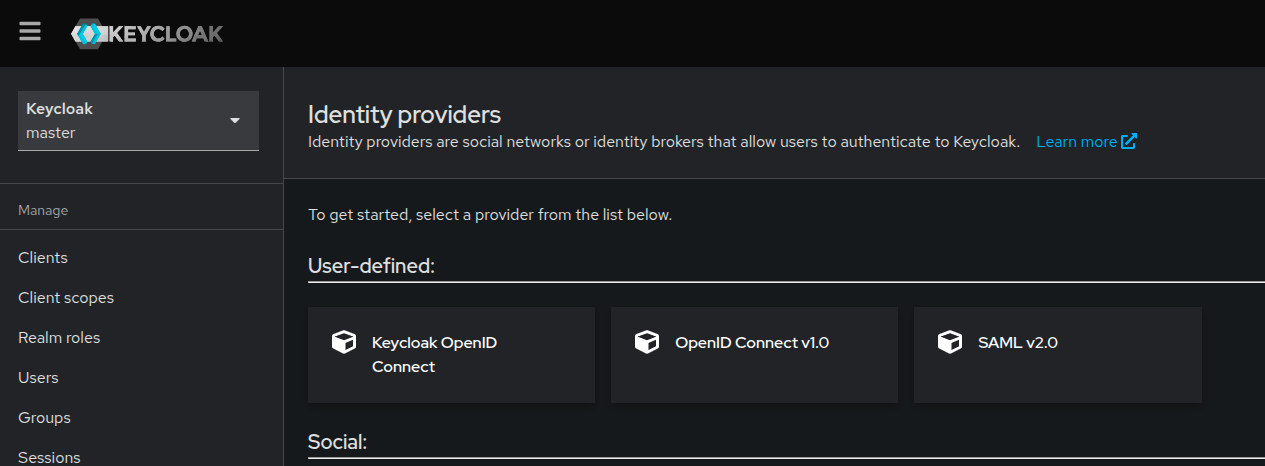
\includegraphics[width=0.9\linewidth]{screenshot007}
		\caption{Protokolle für IdPs in Keycloak}
		\label{fig:screenshot007}
	\end{figure}
	
	\vspace{0.5em}
	\textbf{Grant Typen und Authentifizierungsflüsse:}\\
	Keycloak unterstützt verschiedene \textit{Grant Types}, die beschreiben, wie sich Benutzer oder Clients authentifizieren:
	
	\begin{itemize}
		\item \textbf{Authorization Code Grant:} Benutzer wird zur Keycloak-Loginseite weitergeleitet. Nach erfolgreicher Authentifizierung erhält der Client einen Authorization Code, den er gegen ein Access Token eintauscht. Das Passwort wird dabei nie an die Client-Anwendung weitergegeben.
		\item \textbf{Client Credentials Grant:} Wird für Clients ohne Benutzerinteraktion verwendet. Der Client authentifiziert sich mit seiner Client-ID und einem geheimen Schlüssel (Client Secret), um ein Access Token zu erhalten.
	\end{itemize}
	
	Die \textbf{Client Authentifizierungsmethode} legt fest, wie der Client gegenüber dem Server seine Identität nachweist – z.\,B. mittels Client Secret oder Zertifikat. Während der Grant-Typ die Art der Anmeldung bestimmt, definiert die Client-Authentifizierungsmethode die technische Form des Identitätsnachweises.
	
	Zusätzlich existieren in Keycloak sogenannte \textit{Authentication Flows}, die den Ablauf der Authentifizierung steuern:
	
	\begin{itemize}
		\item \textbf{Standard Flow:} Meist Authorization Code Grant mit Weiterleitung zur Login-Seite.
		\item \textbf{Implicit Flow:} Gibt direkt ein Token zurück, wird aber aus Sicherheitsgründen nicht mehr empfohlen.
		\item \textbf{Direct Access Grant:} Direkte Anmeldung über Benutzername und Passwort, z.\,B. bei Skripten oder mobilen Apps.
		\item \textbf{Device Authorization Grant:} Für Geräte ohne Eingabemöglichkeit, z.\,B. Smart TVs.
		\item \textbf{CIBA (Client-Initiated Backchannel Authentication):} Asynchrone Authentifizierung, z.\,B. über Push-Benachrichtigungen.
	\end{itemize}
	
	\begin{figure}[H]
		\centering
		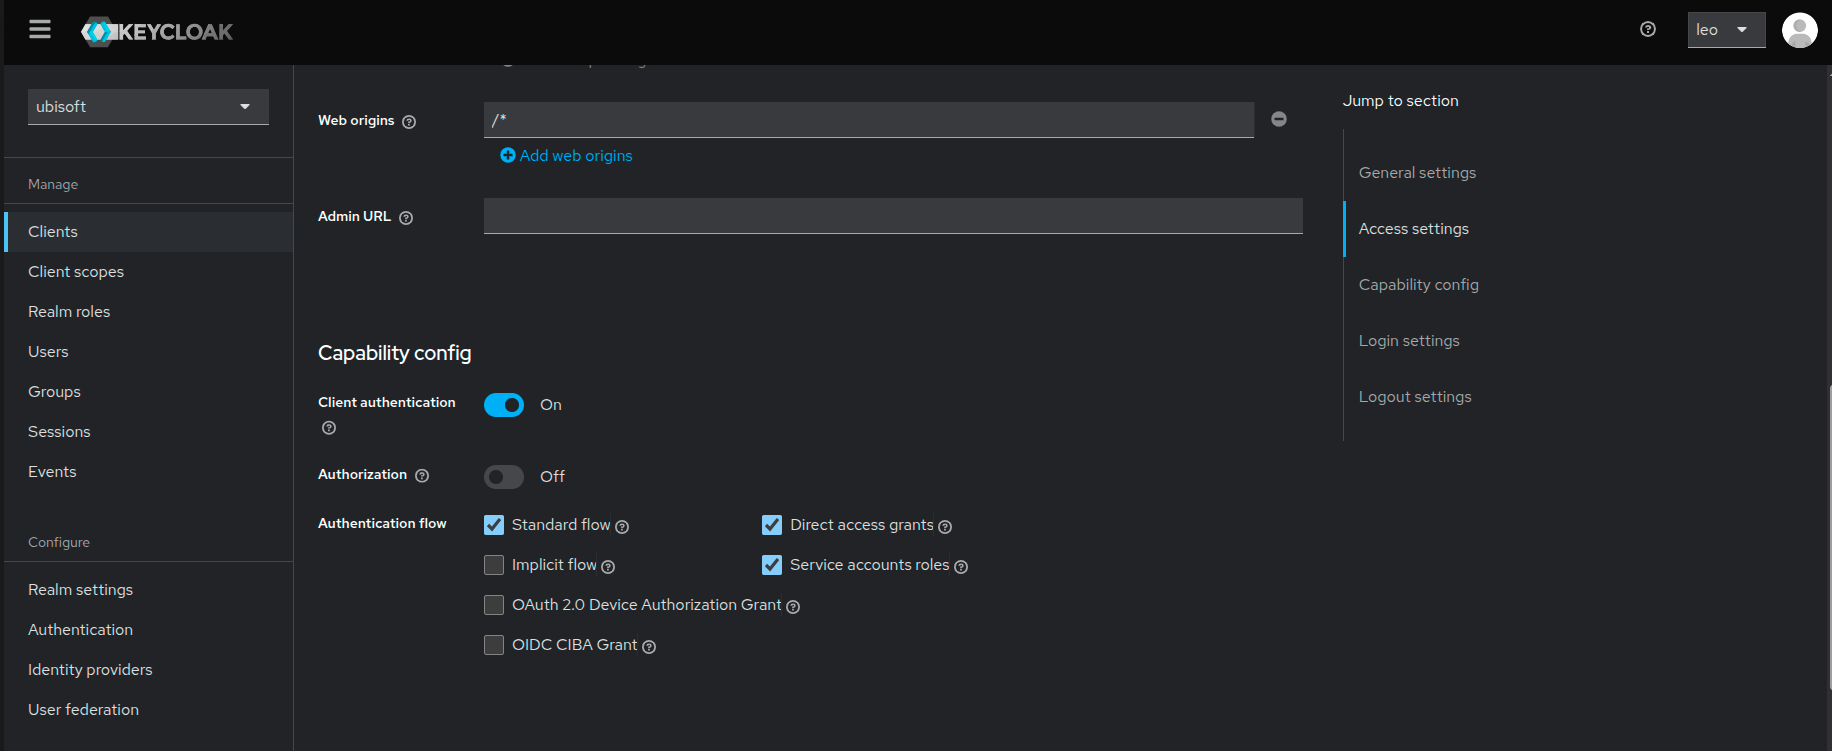
\includegraphics[width=0.9\linewidth]{screenshot013}
		\caption{Beispielhafte Konfiguration von Authentication Flows in Keycloak}
		\label{fig:screenshot013}
	\end{figure}
	
	\vspace{0.5em}
	\textbf{Client-Scope:}\\
	Der \textit{Client-Scope} definiert, welche Benutzerdaten in das Token aufgenommen werden, wenn sich ein Benutzer über einen Client anmeldet. Typische Informationen sind Name, Nachname und E-Mail. Diese Daten werden verschlüsselt übertragen, jedoch besteht ein gewisses Risiko bei Missbrauch oder Diebstahl des Tokens.
	
	\vspace{0.5em}
	\textbf{Rollenmodell:}\\
	Keycloak unterscheidet zwei zentrale Rollentypen:
	
	\begin{itemize}
		\item \textbf{Realm-Rollen:} Gelten global innerhalb eines Realms. Sie eignen sich für übergreifende Rechte, z.\,B. „admin“ für alle Clients.
		\item \textbf{Client-Rollen:} Spezifisch für einen einzelnen Client. Sie erlauben feinere Zugriffskontrolle innerhalb der jeweiligen Anwendung.
	\end{itemize}
	
	\vspace{0.5em}
	\textbf{Service Account Roles:}\\
	Clients können sich in Keycloak auch selbst authentifizieren – ohne Benutzerinteraktion. Wird die \textit{Service Account}-Funktion für einen Client aktiviert, erhält dieser ein eigenes Servicekonto. Dieses Konto kann mit Rollen ausgestattet werden, um Rechte auf bestimmte Ressourcen oder Operationen zu erhalten – z.\,B. für automatisierte Backend-Operationen.
	
	\subsection{Komponenten der Log-Erzeugung}
	Keycloak generiert Logs über eine Kombination aus verschiedenen Frameworks und Komponenten. Grundlage bildet das Logging-Framework von JBoss, wobei moderne Versionen von Keycloak zusätzlich auf das Quarkus-Framework setzen.
	\vspace{0.5em}
	\textbf{Von WildFly zu Quarkus – Technologiewechsel:}\\
	Ursprünglich basierte Keycloak auf dem \textbf{WildFly}-Anwendungsserver\footnote{\url{https://www.wildfly.org/}}, der wiederum die \textbf{JBoss Logging}-Infrastruktur verwendet. Ab Keycloak Version 17 wurde WildFly durch das \textbf{Quarkus}-Framework ersetzt – ein modernes Java-Framework, das speziell für containerisierte und cloud-native Anwendungen entwickelt wurde. Quarkus unterstützt ebenfalls JBoss Logging, sodass bestehende Logging-Mechanismen weiterhin funktionieren.
	
	\begin{figure}[H]
		\centering
		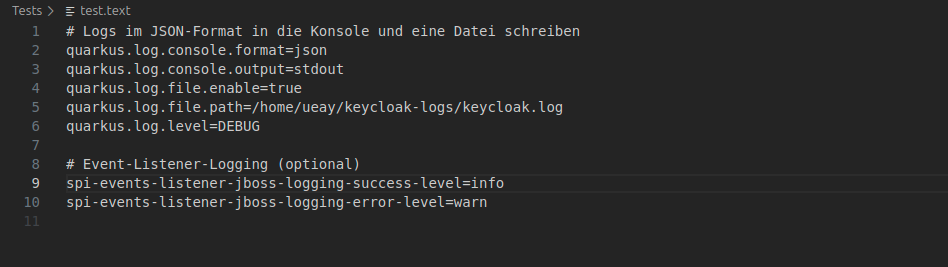
\includegraphics[width=0.9\linewidth]{screenshot008}
		\caption{Beispiel: Aktivierung von Quarkus-Logging in der Keycloak-Konfiguration}
		\label{fig:screenshot008}
	\end{figure}
	
	\vspace{0.5em}
	\textbf{Rolle von JBoss Logging:}\\
	JBoss Logging dient in Keycloak als zentrale Logging-API. Es abstrahiert verschiedene Logging-Backends (wie \texttt{log4j}, \texttt{JUL}, \texttt{Slf4j}) und ermöglicht die strukturierte Ausgabe sicherheitsrelevanter Informationen – z.\,B.:
	\begin{itemize}
		\item \texttt{Realm-ID}
		\item \texttt{Benutzer-ID}
		\item \texttt{IP-Adresse}
		\item \texttt{Event-Typ}
	\end{itemize}
	
	Der Vorteil liegt in der Flexibilität: Entwickler müssen sich nicht auf ein spezifisches Logging-Backend festlegen, sondern können über die einheitliche JBoss-API verschiedene Ausgabekanäle konfigurieren (Konsole, Datei, syslog etc.).
	
	\vspace{0.5em}
	\textbf{Warum nicht Log4j, Logback oder JUL?}\\
	Obwohl es im Java-Ökosystem viele Logging-Frameworks gibt, verzichtet Keycloak bewusst auf deren direkte Verwendung:
	\begin{itemize}
		\item \textbf{Log4j / Logback:} Mächtig, aber externe Abhängigkeiten und teils Sicherheitsrisiken (z.\,B. Log4Shell).
		\item \textbf{JUL (java.util.logging):} Eingebaut, aber funktional begrenzt.
		\item \textbf{Slf4j:} Nur eine Fassade – erfordert Backend wie Logback oder Log4j.
		\item \textbf{System.out / System.err:} Nicht strukturiert, ungeeignet für produktive Logs.
	\end{itemize}
	
	\begin{figure}[H]
		\centering
		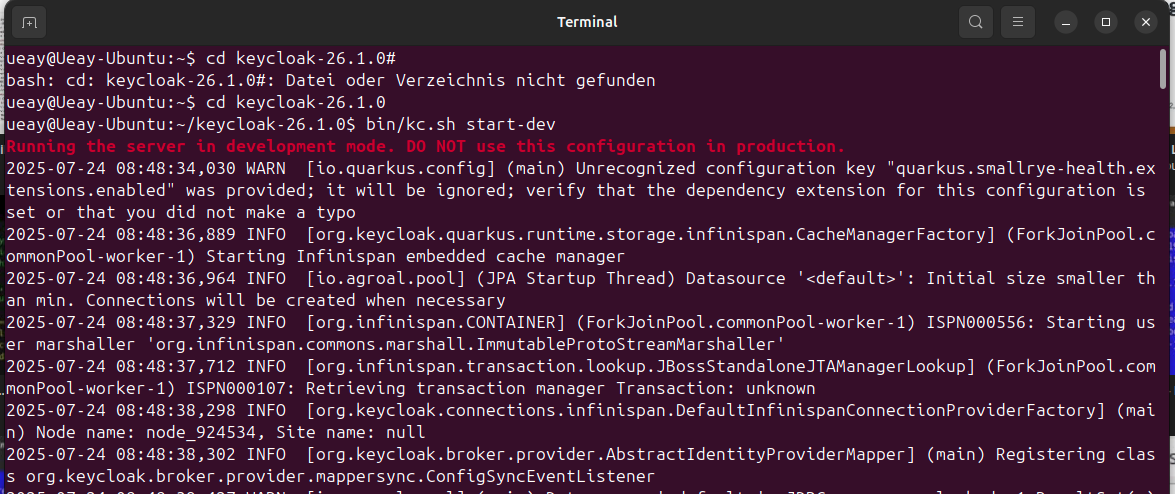
\includegraphics[width=1.1\linewidth]{screenshot014}
		\caption{Log-Ausgaben, wie sie in einer Quarkus-basierten Keycloak-Instanz erzeugt werden}
		\label{fig:screenshot014}
	\end{figure}
	
	\vspace{0.5em}
	\textbf{Vorteile der aktuellen Logging-Architektur:}
	\begin{itemize}
		\item \textbf{Nahtlose Integration:} JBoss Logging ist direkt in Quarkus und die Keycloak-Architektur eingebettet.
		\item \textbf{Sicherheitskontext:} Strukturierte Logs enthalten kontextuelle Daten, die für Auditing und Sicherheitsanalysen wichtig sind.
		\item \textbf{Zentrale Konfiguration:} Log-Level, Ausgabeformate und Ziele können zentral über Konfigurationsdateien gesteuert werden.
		\item \textbf{Konsistenz:} Einheitliches Logging-Verhalten über alle Komponenten hinweg.
	\end{itemize}
	
	Insgesamt stellt JBoss Logging in Kombination mit Quarkus eine robuste, flexible und erweiterbare Logging-Lösung dar, die sowohl Sicherheitsanforderungen als auch Betriebsanforderungen gerecht wird.
	Ein weiterer Baustein ist SLF4J (Simple Logging Facade for Java), das vor allem in vielen externen Bibliotheken der Java-Welt als Logging-Fassade genutzt wird. Quarkus unterstützt SLF4J indirekt, indem es mit einem passenden Backend wie logback oder log4j2 kombiniert werden kann. In Keycloak selbst wird SLF4J jedoch nicht direkt verwendet, da stattdessen vollständig auf JBoss Logging gesetzt wird.
	\vspace{0.5em}
	Für erweiterte oder spezielle Logging-Anforderungen lassen sich Frameworks wie Log4j2 oder Logback über Custom Extensions oder SPIs einbinden. Diese sind nicht standardmäßig in Keycloak aktiv, können aber in Eigenentwicklungen verwendet werden – etwa wenn besondere Formatierungen oder externe Integrationen erforderlich sind.
	\vspace{0.5em}
	Einfache Ausgaben über System.out oder System.err kommen in Keycloak kaum zum Einsatz und dienen allenfalls zu Debug-Zwecken in sehr frühen Initialisierungsphasen. Für produktive Umgebungen sind sie ungeeignet, da sie weder strukturiert noch steuerbar sind und nicht in zentrale Log-Management-Systeme integriert werden können.
	\vspace{0.5em}
	Besonders nützlich ist die Möglichkeit, JSON-basiertes Logging in Quarkus zu aktivieren. Dadurch lassen sich strukturierte Logdaten erzeugen, die sich ideal für den Einsatz in zentralisierten Logging-Stacks wie ELK (Elasticsearch, Logstash, Kibana) oder Loki mit Grafana eignen. Die JSON-Ausgabe wird direkt über eine Property aktiviert (quarkus.log.console.json=true).
	\vspace{0.5em}
	Neben dem klassischen System-Logging bietet Keycloak ein eigenes Audit- und Event-Logging-Subsystem, das unabhängig vom allgemeinen Logsystem funktioniert. Mithilfe des EventListener-SPI können verschiedene Ereignisse – etwa Admin-Änderungen oder Benutzeraktionen – gezielt erfasst werden. Die Ausgabe kann dabei in Form einfacher Logs, in Syslog-Formate oder in benutzerdefinierte Kanäle erfolgen.
	\vspace{0.5em}
	Abschließend unterstützt Keycloak die Integration in externe Logging-Systeme durch Syslog oder Remote Logging. So lassen sich Logs über Tools wie Filebeat an zentrale Systeme weiterleiten (z.B. Logstash oder Cloud-Dienste wie AWS CloudWatch, Google Stackdriver oder Azure Monitor) oder Kubernetes. Dies ist insbesondere in containerisierten oder skalierenden Cloud-Umgebungen entscheidend für Monitoring, Fehleranalyse und Sicherheitsüberwachung.
	
	\subsection{Log-Dateien in Keycloak}
	Logging, bzw. Protokollierung ist ein essentieller Bestandteil für die Überwachung von IT-Systemen. Für das IT-Monitoring dienen Logs zur Verhinderung und Detektion von Anomalien, sei es im Netzwerk, in einem IoT-Gerät oder eben in IAM-Tools. 
	\\[0.5em]
	In Keycloak werden verschiedene Log-Arten unterteilt, wobei die Logs für das Netzwerk, die Access Logs u.A. nicht direkt zu Keycloak gehören.
	Kecyloak unterteilt Logs in folgende Kategorien:
	\begin{itemize}
		\item Server-Logs: Betriebsstatus, Fehler, Debugging-Infos
		\item Event-Logs: Benutzer- und Admin-Events (Event-System)
		\item Audit-Logs: Nachvollziehbarkeit von Änderungen (Admin Events)
		\item Access Logs: Zugriffsversuche und HTTP-Statuscodes (HTTP Layer / Reverse Proxy)
		\item Security Logs: Sicherheitsrelevante Ereignisse und Warnungen
		\item Custom Logs: Erweiterungen und Plugins können eigene Logs erzeugen (SPI)
	\end{itemize}
	Die Logs werden dabei von unterschiedlichen Instanzen in Keycloak erzeugt. Die Server-Logs werden  vom Keycloak-Server selbst erzeugt und weisen die Kategorie \textit{org.keycloak.services} auf. Sie werden mit dem Quarkus-Framework erzeugt.
	\\[0.5em]
	Event-Logs und Audit Logs werden vom Event-System in Keycloak erzeugt, der unter der Kategorie \textit{org.keycloak.events} zu erkennen ist.
	\\[0.5em]
	Access Logs werden auf der Anwendungs- und Netzebene erzeugt- hauptsächlich außerhalb Keycloaks und sind gekennzeichnet als \textit{io.quarkus.http}
	\\[0.5em]
	
	\subsection{Event-Logs}
	Analysiert in dieser Arbeit werden die Event-Logs. Grund hierfür ist, dass diese wichtige Features enthalten, welche das Bneutzerverhalten beschreiben. Server-Logs beziehen sich zu sehr auf Netzbasierte Logs und andere Logs, wie Audit-Logs sind Unterkategorien von Events-Logs. Da keine SPI verwendet wird und nur die einzelne Keycloak-Instanz untersucht wird, fallen Custom Logs ebenfalls weg als Teil der Trainingsdaten und Security Logs werden nur erzeugt, wenn es die dazu gehörigen Komponenten dazu gibt,welche hier auch nicht angewandt werden.
	\\[0.5em]
	
	Keycloak unterteilt unter Anderem zwei Arten von Events-Logs:
	
	\begin{itemize}
		\item Admin Logs (Audit Logs)
		\item User Logs (Event Logs)
	\end{itemize}
	
	Die Admin Logs enthalten alle Logs bzgl. den Operationen des Admins und die User Logs nur die Logs von Benutzern, die nicht Admin sein.
	
	\subsection{Aufbau der Event-Logs}
	Folgende Features sind stets in den User Event Logs enthalten:
	
	\begin{itemize}
		\item timestamp
		\item log\_level
		\item category
		\item type
		\item ipAddress
		\item realmName
		\item realmId
		\item clientId
		\item userId
	\end{itemize}
	Man erkennt, dass wichtige Attribute, wie bspw. der Standort des Clients fehlen. Dies liegt an datenschutzrechtlichen Gründen, jedoch erschwert dies Anomalien in den Logs zu erkennen, weil diese anhand des Standortes erkannt werden. Dies muss noch als Störfaktor erkannt werden. Anhand des Standortes können somit schon mal keine Anomalien erkannt werden. Timestamp ist einer der wichtigen Attribute, welche zeigen, um welche Zeit der Log erzeugt wurde. Zur Analyse zeitbasierter Daten eignen sich timestamp als aussagekräftige Information für die LSTM-AE-Hybridmodelle.
	\\[0.5em]
	Desweiteren unterteilt Keycloak noch sogenannte Log-Level. Diese zeigen, ob eine bestimmte Operation erfolgreich war oder nicht oder geben andere Informationen bzgl. einer Operation.
	Bekannte Log-Level sind z.B. INFO, FATAL oder ERROR. Alle Arten finden sich in der Dokumentation \footnote{https://www.keycloak.org/server/logging}.
	Das Loglevel (z.B. FATAL, ERROR, INFO) bestimmt die Art des Logs, z.B. ob es zum Debugging dient oder eine Warnung erschient, entweder ein Fehler oder eine Info.
	\\[0.5em]
	"Category" beschreibt hier die Art des Logs. Da in dieser Arbeit mit Keycloak-Logs gearbeitet wird, kommen insbesondere der JBossLogger \footnote{https://docs.jboss.org/process-guide/en/html/logging.html} und die JPA-Komponente \footnote{https://docs.spring.io/spring-data/jpa/reference/index.html} von Keycloak zum Einsatz.
	\\[0.5em]
	Des weiteren von Bedeutung in den Logs haben die Ereignis-Typen:
	Bspw. ist LOGIN ein Ereignis-Typ bei dem der Benutzer sich anmeldet. Dies wird in Keycloak auch regelmäßig dokumentiert. Andere Ereignistypen sind bspw. TOKEN\_REFRESH, bei dem der Benutzer einen neuen Token bekommt. 
	
	\begin{figure}[H]
		\centering
		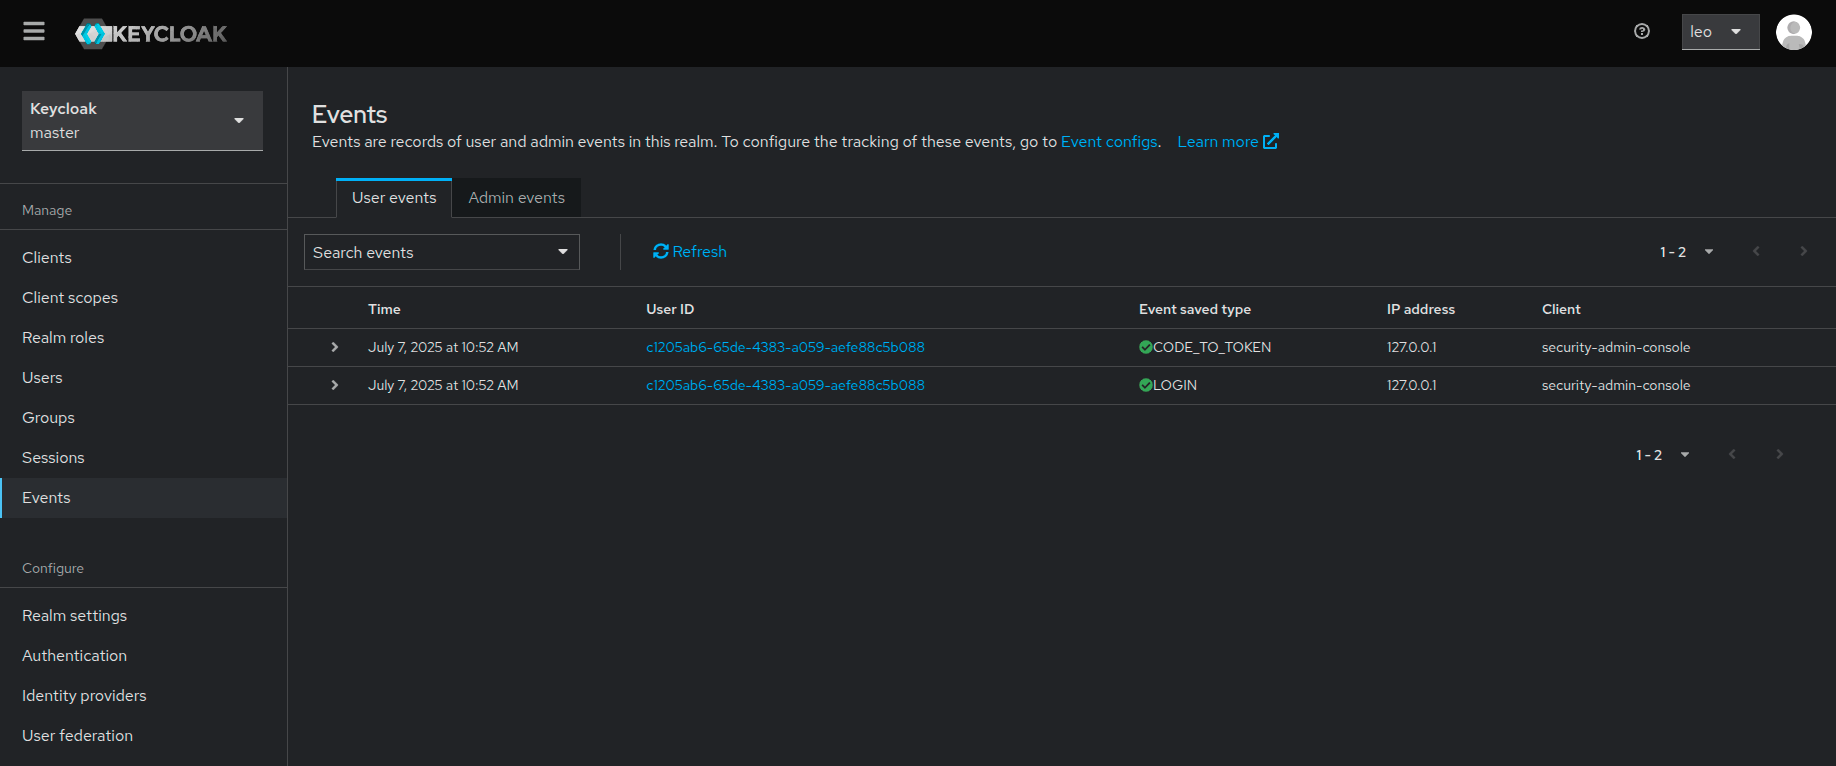
\includegraphics[width=1.0\linewidth]{screenshot002}
		\caption{Beispiel Events nach Eventtyp}
		\label{fig:screenshot002}
	\end{figure}
	
	Je nach Eventtyp werden Features angehängt oder weggelassen, z.B. wird beim Login noch in den Logs die Token-Url, die Art der Verbindung und auch die Art des Authentifizierungsprotokolls angegeben. "Type" steht hier für den Event-Typen. Die wichtigsten Event Type sind dabei folgende:
	
	\begin{itemize}
		\item LOGIN: Log, der generiert wird, wenn sich ein Benutzer erfolgreich einloggt über  Keycloak selbst.
		\item CODE TO TOKEN: Wird erzeugt, sobald der Benutzer sich über seine Anmeldedaten auf dem Keycloak-Server authentifiziert hat und von diesem einen Access Token erhalten hat.
		\item CLIENT LOGIN: Log, der generiert wird, sobald sich der Benutzer über einen Drittanbieter einloggt.
		\item LOGIN ERROR: Fehler beim Login über Keycloak
		\item CODE TO TOKEN ERROR: Anmeldedaten war falsch, Server lehnt Anmeldedaten von Benutzer ab
	\end{itemize}
	
	In den Admin Logs wiederum sind noch Features enthalten, welche in den normalen User Event Logs nicht vorkommen, u.A. 'operationType': Diese beinhalten typische CRUD-Operationen wie UPDATE, CREATE, DELETE und ACTION \footnote{https://github.com/keycloak/keycloak/blob/main/model/jpa/src/main/java/org/keycloak/events/jpa/JpaAdminEventQuery.java}. 
	\\[0.5em]
	
	\section{Theoretischer Hintergrund der Modelle}
	\subsection{LSTM}
	Long Short-Term Memory (LSTM) ist ein Recurrent Neural Network (\gls{rnn}), welches dazu entwickelt wird zeitabhängige Datenabfolgen zu erkennen und zu analysieren \cite{staudemeyer2019understanding}.
	RNNs sind eine spezielle Klasse von neuronalen Netzwerken, welche dazu entwickelt wurden, sequentielle Daten zu verarbeiten, also Daten bei den die Reihenfolge der zu verarbeitenden Daten entscheiden ist. daher eignen sie sich gut Zeitreihen zu analysieren. RNNs können die nacheinander folgenden, abhängigen Daten anhand eines sogenannten Hidden Errors analysieren: Dabei wird im Hidden Error die zuvor analysierten Daten behalten und mit den nächsten Daten in einem gemeinsamen Kontext verarbeitet. Der Hidden State wird bei jedem Zeitschritt aktualisiert und bildet somit einen gemeinsamen Kontext für die Verarbeitung der aktuellen und vorherigen Eingaben.
	Das Problem an RNNs ist jedoch, dass bei längeren Datensequenzen die Erinnerung der zu weit liegenden Daten verblasst.
	LSTMs gleichen diese Nachteile aus: Sie besitzen über eine Zellstruktur, die gewährleistet, dass auch zu alte Datensequenzen noch erinnert werden.
	Dies wird durch diese drei Bestandteile gewährleistet \cite{hochreiter1997long}:
	\begin{itemize}
		\item \textbf{Forget Gate:} Entscheidet, welche Informationen aus der Zellzustand gelöscht werden sollen.
		\item \textbf{Input Gate:}  Steuert, welche neuen Informationen in den Zellzustand aufgenommen werden.
		\item \textbf{Output Gate:} Bestimmt, welche Informationen aus der Zelle als Ausgabe weitergegeben werden.
	\end{itemize}
	LSTM jedoch haben auch ihre Kapazitäten und auch hier können längere Sequenzen trotz diesen Gates für Verarbeitungsschwierigkeiten sorgen.
	Probleme wie das Vergessen weiter zurückliegender Informationen oder eine ineffiziente Nutzung des Speichers können weiterhin auftreten – wenn auch in deutlich abgeschwächter Form im Vergleich zu Standard-RNNs \cite{hochreiter1997long}.
	
	\subsection{Autoencoder}
	Ein Autoencoder ist eine spezielle Form eines neuronalen Netzwerks, das aus zwei Hauptbestandteilen besteht: der Encoder- und der Decoder-Schicht \cite{michelucci2022introduction}.
	\\[0.5em]
	Die Encoder-Schicht komprimiert die Eingabedaten und reduziert ihre Dimensionen auf eine kleinere Repräsentation, die sogenannte Bottleneck-Schicht. Diese Bottleneck-Schicht ist der engste Teil des Netzwerks und zwingt das Modell, die wichtigsten Merkmale der Daten in verdichteter Form zu lernen. Dadurch werden irrelevante oder redundante Informationen herausgefiltert, was den Autoencoder befähigt, die Essenz der Eingabedaten zu erfassen.
	\\[0.5em]
	Die Decoder-Schicht nimmt diese komprimierte Repräsentation und versucht, die ursprünglichen Daten daraus möglichst genau zu rekonstruieren. Das Netzwerk lernt durch Minimierung des Rekonstruktionsfehlers, also der Differenz zwischen Eingabedaten und rekonstruierten Daten.
	\\[0.5em]
	Diese Fähigkeit macht Autoencoder besonders nützlich für Aufgaben wie Anomalieerkennung. Wenn die Rekonstruktion schlecht gelingt (hoher Rekonstruktionsfehler), deutet dies darauf hin, dass die Eingabedaten von den gelernten Mustern abweichen und somit potenziell eine Anomalie darstellen.
	
	\paragraph{Bottleneck und seine Bedeutung}
	Der Bottleneck ist entscheidend, da er die Kapazität des Autoencoders steuert. Ein zu kleiner Bottleneck kann dazu führen, dass wichtige Informationen verloren gehen und die Rekonstruktion schlecht wird. Ein zu großer Bottleneck hingegen erlaubt es dem Netzwerk, einfach die Identität zu lernen und Daten "durchzuschleusen", wodurch der Autoencoder seine Fähigkeit zur Merkmalskompression verliert.
	
	\paragraph{Varianten und Architekturen}
	Neben dem klassischen Autoencoder gibt es weitere Varianten, z.B. den Variational Autoencoder (VAE), der probabilistische Modelle nutzt und generative Fähigkeiten besitzt, oder den Denoising Autoencoder, der lernt, verrauschte Eingaben zu bereinigen. Außerdem können Autoencoder aus mehreren Schichten bestehen (deep Autoencoder), um komplexere Merkmale zu extrahieren.
	
	\paragraph{Vorteile}
	
	Automatische Merkmalsextraktion ohne explizite Label
	
	Gut geeignet für unüberwachte Lernaufgaben
	
	Effiziente Dimensionsreduktion und Datenkompression
	
	\paragraph{Nachteile}
	
	Benötigen große Datenmengen zum Trainieren
	
	Können bei zu großem Bottleneck trivial werden (Identitätsfunktion lernen)
	
	Rekonstruktionsfehler ist nicht immer ein perfekter Indikator für Anomalien, vor allem bei sehr komplexen Daten
	
	Training kann rechenintensiv sein
	
	\paragraph{Anwendungsbereiche}
	Autoencoder finden Anwendung in der Bildkompression, Anomalieerkennung in Netzwerken oder Produktionsprozessen, Feature Learning vor Klassifikationsaufgaben oder generativer Modellierung.
	
	\begin{figure}[H]
		\centering
		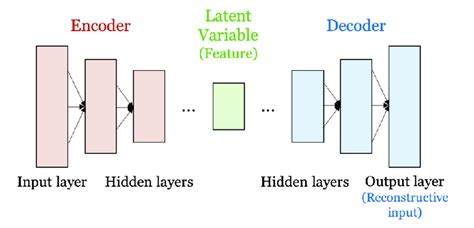
\includegraphics[width=0.7\linewidth]{screenshot004}
		\caption{Visuelle Darstellung der Funktion des AEs, Quelle: https://www.researchgate.net/figure/Structure-of-the-autoencoder\_fig1\_365074431}
		\label{fig:screenshot004}
	\end{figure}
	
	Autoencoder werden für Anomalieerkennung oder auch Dimensionsreduktion verwendet.
	
	\paragraph{Mit dem LSTM kombiniert}
	Autoencoder lassen sich besonders gut mit Long Short-Term Memory (LSTM)-Netzwerken kombinieren, wenn es um sequenzielle oder zeitabhängige Daten geht. Während der klassische Autoencoder oft für statische Daten verwendet wird, können LSTM-Autoencoder zeitliche Abhängigkeiten erfassen und lernen, wie sich Daten über Zeit entwickeln.
	\\[0.5em]
	Ein LSTM-Autoencoder nutzt LSTM-Zellen im Encoder und Decoder, um komplexe zeitliche Muster zu erfassen und zu rekonstruieren. Diese Kombination ist besonders nützlich bei Anomalieerkennung in Zeitreihen, wie etwa in der Überwachung von Maschinenzuständen, Finanzdaten oder Netzwerksicherheit. Anomalien fallen hier oft durch signifikant erhöhte Rekonstruktionsfehler auf, da die zeitlichen Muster nicht gut rekonstruiert werden können.
	\\[0.5em]
	Durch die Fähigkeit von LSTM, langfristige Abhängigkeiten zu modellieren, und die Komprimierung des Autoencoders entsteht ein mächtiges Werkzeug für die Analyse und das Verständnis komplexer, sequenzieller Daten.
	
	\subsection{Isolation Forest}
	Isolation Forest ist ein unüberwachter Lernalgorithmus, welcher durch Partitionen Daten voneinander trennen kann, indem er binäre Bäume erzeugt. Er unterteilt die Daten so lange, bis keine Isolierung der Daten mehr möglich ist. Durch dieses Vorgehen lasen sich auch Anomalien erkennen: Die Anomalien werden je danach erkannt, wie isoliert die Daten eingeteilt wurden. Je isolierter die Datenpunkte aufgeteilt wurden, desto wahrscheinlicher ist es, dass es eine Anomalie ist. Wenn sich Datenpunkte in ihrer Form ähneln, so würde der Algorithmus diese nicht zu stark isolieren. Lassen sich diese jedoch stark anhand ihrer Merkmale isolieren, so  ist es wahrscheinlicher, dass diese keiner üblichen Menge eingeteilt werden kann \cite{liu2008isolation}.
	\\[0.5em]
	\begin{figure}
		\centering
		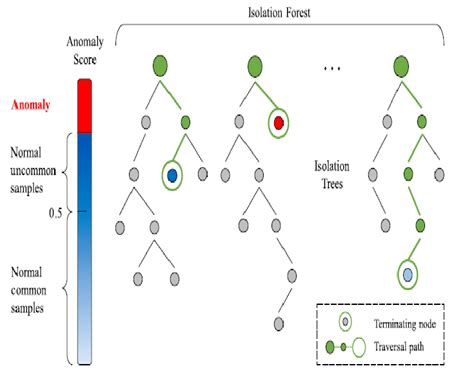
\includegraphics[width=0.7\linewidth]{screenshot005}
		\caption{Visuelle Darstellung der Funktion des AEs, Quelle: https://www.researchgate.net/figure/Anomaly-Detection-using-Isolation-Forest-18\_fig3\_350551253}
		\label{fig:screenshot005}
	\end{figure}
	
	Der Algorithmus erzeugt Isolation Trees, welche aus Blattknoten oder aus einem inneren Knoten besteht,d er eine Testregel enthält, die die Daten in zwei Gruppen aufteilt. Die Testregel besteht aus einem Wert aus der Auswahl eines Merkmals  q und einem Schwellenwert p, so dass alle Datenpunkte, deren Wert für q kleiner als p ist, in den linken Kindknoten kommen, und alle anderen in den rechten Kindknoten.
	\\[0.5em]
	Zum Aufbau eines solchen Baums nimmt man eine Stichprobe von Datenpunkten und teilt sie rekursiv auf, indem man zufällig ein Merkmal und einen Split-Wert auswählt. Dieser Prozess wird so lange wiederholt, bis
	eine maximale Baumhöhe erreicht ist, nur noch ein Datenpunkt übrig ist, oder
	alle Datenpunkte im aktuellen Teilbaum identisch sind \cite{liu2008isolation}.
	\\[0.5em]
	Das Ergebnis ist ein vollständiger binärer Baum, bei dem jeder Datenpunkt in einem Blattknoten isoliert wird.
	\\[0.5em]
	Wenn alle Datenpunkte unterschiedlich sind, dann gilt:
	\begin{itemize}
	\item Es gibt genauso viele Blätter wie Datenpunkte (n).
	
	\item Die Anzahl der inneren Knoten ist n - 1.
	
	\item Insgesamt hat der Baum 2n - 1 Knoten.
	
	\item Der Speicherbedarf wächst also linear mit der Anzahl der Datenpunkte.
	\end{itemize}
	
	Isolation Forest unterteilt jedoch zufällig die Datenpunkte, wobei man die Sinnhaftigkeit des Algorithmus hinterfragen kann.
	
	\subsection{One-Class SVM}
	One-Class Support Vector Machine ist ein unüberwachter Lernalgorithmus, welcher durch die Erstellung von Ebenen Datenpunkte klassifizieren kann. Oder wie es Kun-Lun Li et Al. zitieren \cite{li2003improving}:
	"Bei nichtlinear trennbaren Daten können wir sie durch eine nichtlineare Abbildung in einen hochdimensionalen Raum transformieren, so dass die Daten Punkte linear trennbar sind."
	\\[0.5em]
	\begin{figure}
		\centering
		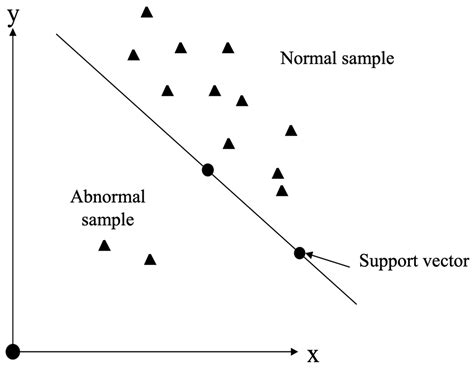
\includegraphics[width=0.7\linewidth]{screenshot006}
		\caption{Visuelle Darstellung  OCSVM. Quelle: https://www.mdpi.com/2076-3417/13/3/1734}
		\label{fig:screenshot006}
	\end{figure}
	
	\gls{ocsvm} beginnt zuerst eine Hyperebene zu definieren, welche den Nullpunkt im Raum trennt. Die Ebene wird so gebildet,dass auf der einen Seite die Daten und auf der anderen Seite die Zielwerte liegen. Der Nullpunkt,also der Ursprung stellt dabei die andere Seite dar. Dies ist räumlich durch den Gaussian RBF Kernel möglich, welcher alle Daten auf einer Kugel abbildet, wobei der Ursprung dort zentriert ist. Ein Problem,dass sich hie ergibt, ist dass der Ursprung den Raum für die Anomalien abbildet, obwohl das in de Realität so ist \cite{bounsiar2025oneclass}.
	
	\subsection{DBSCAN}
	DBSCAN ist ein dichtebasiertes Cluteringverfahren, dass Datenpunkte anhand ihrer Dichte zu anderen Punkten klassifizieren kann.
	Die Dichte wird durch die Anzahl der Nachbarpunkte innerhalb eines Radius (Eps) gemessen, wobei mindestens eine Mindestanzahl von Punkten (MinPts) in diesem Radius vorhanden sein muss \cite{ester1996dbscan}. Die Wahl dieser Parameter ist entscheidend für den Erfolg der Klassifizierung.
	
	\begin{figure}[H]
		\centering
		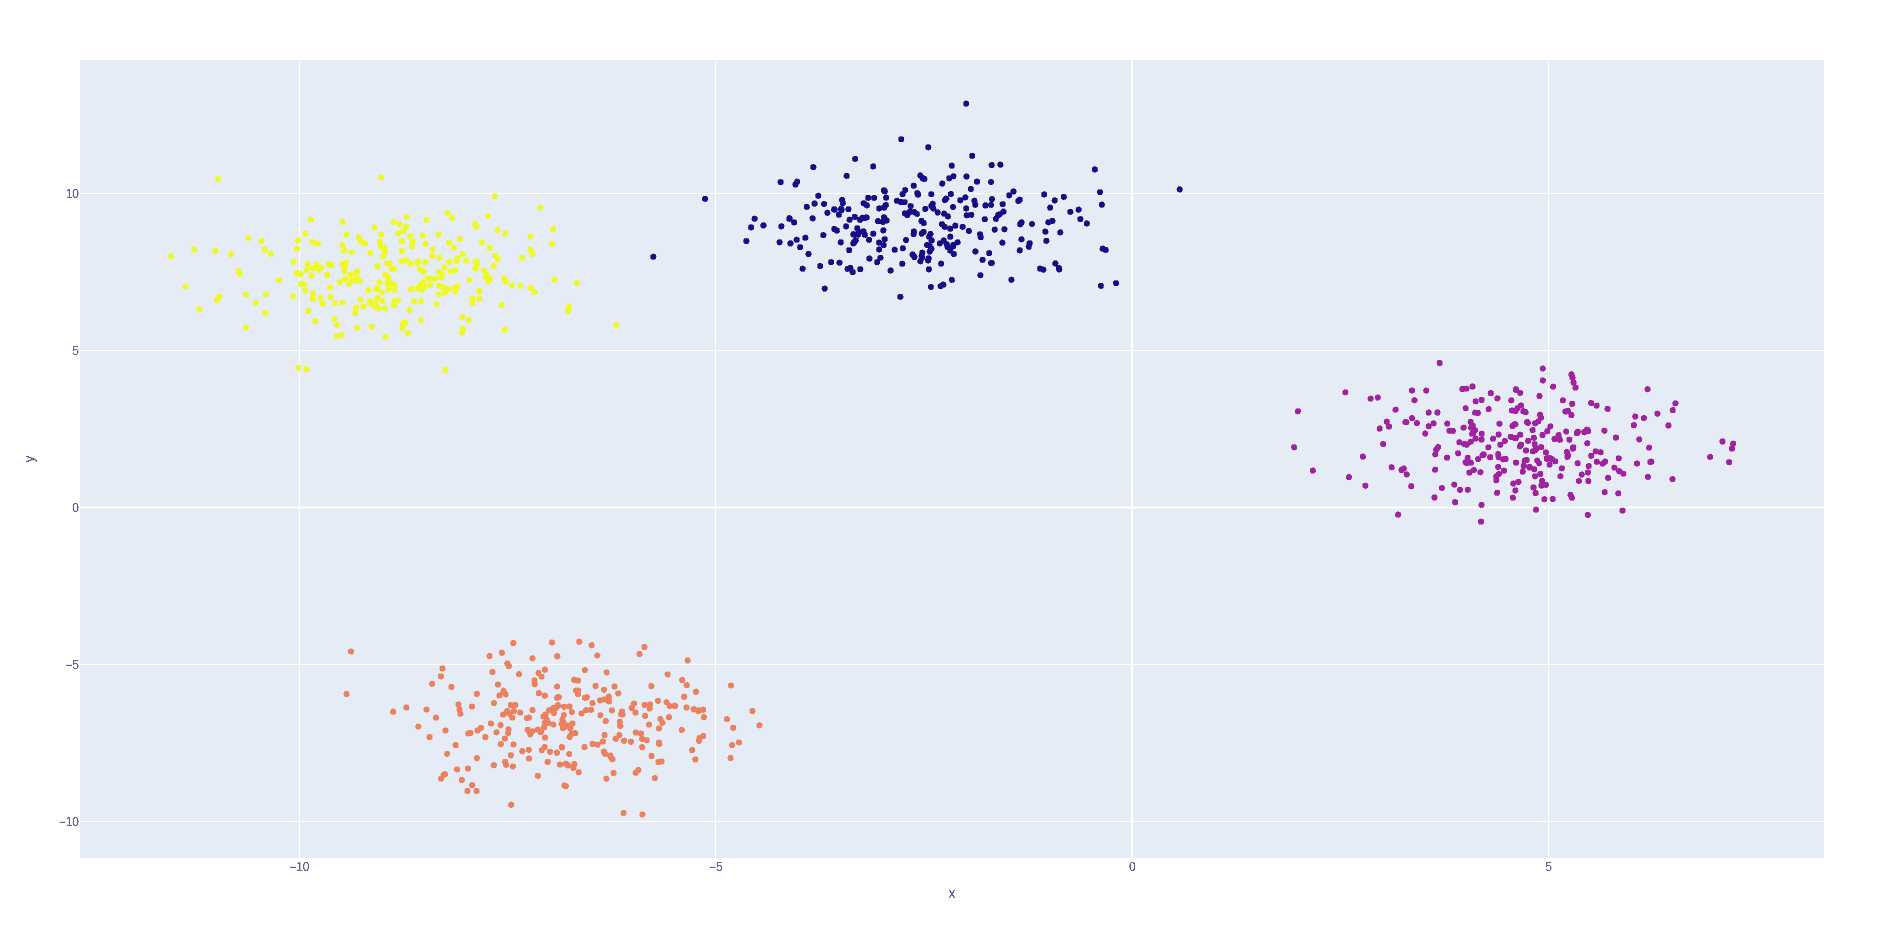
\includegraphics[width=0.9\linewidth]{screenshot015}
		\caption{Beispiel DBSCAN-Cluster, Quelle: \url{https://www.baeldung.com/wp-content/uploads/sites/4/2023/04/clusters.png}}
		\label{fig:screenshot015}
	\end{figure}
	
	Der Algorithmus läuft folgendermaßen ab:
	Man startet von einem bestimmten Punkt p. Daraufhin werden alle Punkte gesucht, welche sich in der Nähe von p befinden. Sobald eine Mindestanzahl von Eps erreicht ist, die auch durch MinPts festgelegt wird, so bildet sich ein Cluster. Danach werden alle Punkte die nun zu einem Cluster gehören, aus einer Liste an verbleibenden Punkten herausgenommen. Daraufhin wird p zufällig an einen weiteren Ort im Raum platziert, wo noch kein Cluster gebildet wurde. Dies geschieht solange, bis keine Punkte in der Liste übrig sind. Die restlichen Punkte, die keinem Cluster zugeordnet sind, heißen Noises. Wenn es zu viele Noises gibt, heisst das, dass nicht effizient klassifiziert wurde \cite{ester1996dbscan}. 
	
	\subsection{Alternative Algorithmen}
	Wie im Forschungsstand bereits erwähnt, wurde auch in Erwägung gezogen, anstelle von DBSCAN das hierarchische Verfahren HDBSCAN (Hierarchical Density-Based Spatial Clustering of Applications with Noise) zu verwenden. Letztlich wurde jedoch darauf verzichtet, obwohl HDBSCAN im Vergleich zu DBSCAN in vielerlei Hinsicht robuster ist – insbesondere bei der Identifikation von Clustern in hochdimensionalen oder verrauschten Daten. HDBSCAN hat den Vorteil, dass es keine globale Dichte-Schwelle voraussetzt und sich besser an lokale Strukturen anpassen kann. Ein Grund für den Verzicht auf HDBSCAN ist jedoch die derzeit noch begrenzte Anzahl an Studien und Erfahrungswerten in konkreten Anwendungskontexten. Im Gegensatz dazu existiert zu DBSCAN eine Vielzahl an Veröffentlichungen, auf die man sich bei der Modellentwicklung stützen kann. Es wäre durchaus denkbar, HDBSCAN in Kombination mit LSTM-Autoencodern (LSTM-AE) in einer eigenständigen Bachelorarbeit weiterführend zu untersuchen.
	\\[0.5em]
	Auch andere Verfahren wie K-Means oder LOF (Local Outlier Factor) wurden in Betracht gezogen. Diese sind grundsätzlich zur Anomalieerkennung geeignet, insbesondere in kleineren oder stärker strukturierten Datensätzen. Jedoch stoßen beide Methoden bei großen, komplexen oder verrauschten Datenmengen schnell an ihre Grenzen: K-Means ist empfindlich gegenüber Ausreißern und setzt eine feste Clusteranzahl voraus, während LOF mit zunehmender Datenmenge schnell ineffizient wird. LOF identifiziert Anomalien, indem es die lokale Dichte eines Punkts mit der seiner Nachbarn vergleicht – weicht sie stark ab, wird der Punkt als potenzieller Ausreißer markiert.
	
	\section{Implementierung}
	\subsection{Hybridmodelle mit LSTM-AE}
	Generell wurden die Modelle nach der selben Architektur gebaut:
	
	\begin{figure}[H]
		\centering
		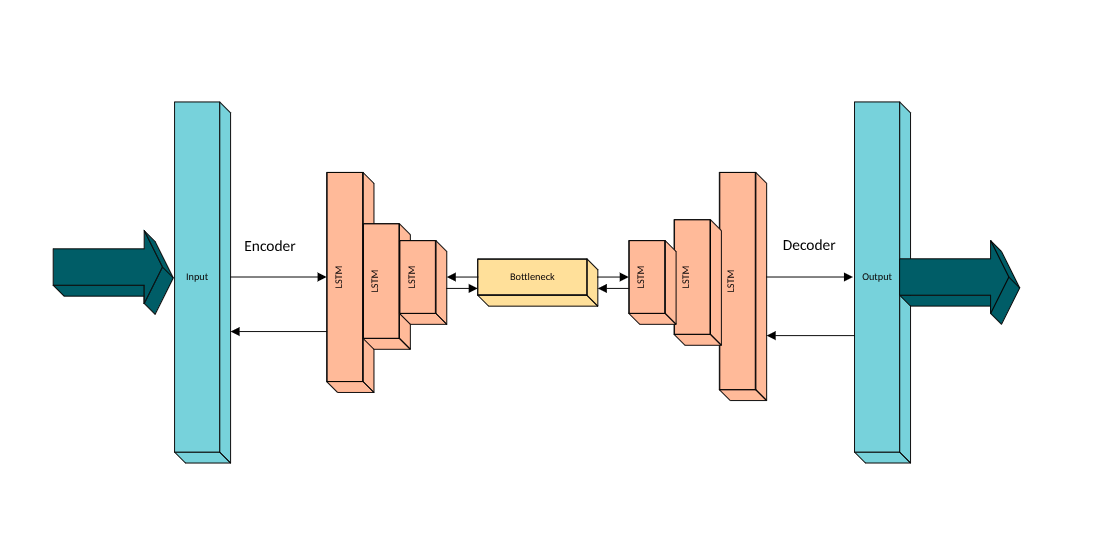
\includegraphics[width=0.7\linewidth]{screenshot001}
		\caption{Architektur}
		\label{fig:screenshot001}
	\end{figure}
	
	Die Logs werden separat je nach Training, Test und Validierung in Dateien gepackt und dann zu Beginn ausgelesen. Zuerst werden diese Daten vorverarbeitet. Die Features werden danach automatisch in numerische, kategorische oder nicht definierte Daten eingeteilt. Es erfolgt dabei nicht sowie üblich Überprüfungen auf NaN oder None- da diese zur Anomalie-Erkennung beitragen und stattdessen als ein Ersatzwert definiert werden statt sie komplett zu entfernen. NaN-Werte können bspw. bei falschen Accounts oder vielleicht bei Bots auftreten, weshalb es wichtig ist, diese in der Analyse beizubehalten. Die eingeteilten und bereinigten Daten werden danach wieder zusammengefügt. Alle drei Dateien, also Evaluierungs-, Test- und Trainingsdateien werden dabei einzeln bereinigt und zusammengefügt. Darauf hin werden alle Daten mit der standardisiert und skaliert. Da der LSTM-AE nur mit sequentiellen Daten arbeiten kann, wurden diese Dateien in Sequenzen aufgeteilt.
	\\[0.5em]
	Es wurden folgende Parameter bestimmt:
	
	\begin{table}[h]
		\centering
		\begin{tabular}{ll}
			\toprule
			\textbf{Parameter}       & \textbf{Wert}            \\
			\midrule
			seq\_length             & 15                       \\
			batch\_size             & 128                      \\
			encoder\_layers         & [1024, 512, 256]         \\
			decoder\_layers         & [256, 512, 1024]         \\
			dropout\_rate           & 0.2                      \\
			learning\_rate          & 0.0001                   \\
			\bottomrule
		\end{tabular}
		\caption{Bestimmte Parameter der Modellkonfiguration}
		\label{tab:model_params}
	\end{table}
	
	\subsubsection{Implementierung: Isolation Forest}
	Die Trainingsfehler, also die Daten, welche nicht klar klassifiziert werden konnten, werden danach jeweils mit einem der vorimplementierten Modelle trainiert. Im Fall des Isolation Forest wird ein auf Entscheidungsbäumen basierender Algorithmus genutzt, der speziell für die Erkennung von Ausreißern in hochdimensionalen Daten entwickelt wurde. Dabei wird das Modell auf den Fehlerwerten der Trainingsdaten fitten, um anschließend auf die Testdaten angewendet zu werden. Die Vorhersage klassifiziert dabei jeden Datenpunkt als normal (1) oder anomal (-1). Diese Ergebnisse werden binär kodiert, um eine einfache Auswertung zu ermöglichen. Da die zugrunde liegenden Daten sequenzbasiert aufgebaut sind – beispielsweise aus Zeitreihen bestehen – wird zusätzlich ein Abgleich mit den tatsächlichen Labeln vorgenommen. Hierzu wird aus den Zielwerten der Testdaten die letzte Klasse jeder Sequenz extrahiert, um sie mit den Vorhersagen vergleichen zu können.
	
	\subsubsection{Implementierung: OCSVM}
	Für die Umsetzung der One-Class SVM wird das Modell mit einem sehr niedrigen nu-Wert von 0.005 initialisiert. Dieser Wert steuert die erwartete Rate an Ausreißern im Trainingsdatensatz. Zusätzlich wird der Parameter gamma auf 50 gesetzt, was die Einflussweite einzelner Datenpunkte auf die Entscheidungsgrenze definiert. Anschließend wird das Modell mit den Fehlerwerten der Trainingsdaten trainiert, die zuvor durch ein Rekonstruktionsmodell (z.\,B. LSTM-Autoencoder) erzeugt wurden.Nach dem Training wird die One-Class SVM auf die Fehler der Testdaten angewendet. Die Methode predict() liefert Vorhersagen in Form von 1 (normal) oder -1 (anomal). Diese Vorhersagen werden daraufhin in binäre Werte (1 = Anomalie, 0 = normal) umgewandelt. Um die Klassifikation korrekt auszuwerten, wird wie auch bei den anderen Verfahren für jedes Sequenzfenster das zugehörige Label aus den ursprünglichen Testlabels extrahiert. Daraus entsteht ein Label-Vektor, der mit den Vorhersagen verglichen wird.
	
	\subsubsection{Implementierung: DBSCAN}
	Im Fall von DBSCAN handelt es sich um ein dichtebasiertes Clusteringverfahren, das keine explizite Trainingsphase benötigt. Das Modell wird direkt auf die Fehlerwerte der Testdaten angewendet. Als Parameter wird eps = 0.05 gewählt, um die maximale Nachbarschaftsdistanz für die Punkte zu begrenzen, sowie min\_samples = 40, was die Mindestanzahl an Nachbarn definiert, um als Kernpunkt eines Clusters zu gelten. Die Methode fit\_predict() gibt für jeden Punkt entweder eine Clusterzuweisung (0, 1, …) oder -1 zurück – letzteres kennzeichnet Datenpunkte, die als Rauschen bzw. Anomalien erkannt wurden.
	Analog zu den anderen Verfahren werden die -1-Werte in binäre Anomalien umgewandelt. Die tatsächlichen Labels werden erneut sequenzbasiert aus dem vollständigen Label-Vektor extrahiert. Abschließend wird ein Classification Report erzeugt, um die Qualität der durch DBSCAN erkannten Anomalien gegenüber den echten Anomalien zu evaluieren.
	
	\subsection{Alternative Architekturen}
	Es bestand die Möglichkeit, vorher eines der Algorithmen zu trainieren und danach die selben Daten nochmals in den LSTM-AE. Es ist also der umgekehrte Weg, welcher auch in einer Masterabeit verwendet wurde, bei dem ein Hybridmodell zwischen IF und LSTM-AE erstellt wurde \cite{hybrid_if_lstm2023}.
	Desweiteren gibt es auch Architekturen, welche nur DBSCAN und OCSVM benutzen, wobei die Daten zuerts von OCSVM verwendet werden und später durch DBSCAN geclusert werden.
	\\[0.5em]
	Es gab auch Ideen, für größerer Hybridmodelle. U.A. wurde eine große Kombination aus LSTM-AE, DBSCAN und IF erstellt. Die Daten werden demnach zuerst vom LSTM-AE verarbeitet. Die Fehler daraus werden geclustert durch DBSCAN, falls es auch unterschiedliche Fehlerarten gibt. schlussendlich entschiedet IF, welche Anormal sind und welche nicht.
	\\[0.5em]
	Diese Alternativen wurden jedoch nicht umgesetzt, da sie zu komplex sind, insbesondere, weil in dieser Arbeit nur verhaltensbasierte Anomalien verarbeitet werden, welche sich in Event-Logs zeigen. Solch ein komplexes Modell wurde auch erwogen, weil zu Beginn diskutiert wurde, Modelle in Cloud-Umgebungen zu verwenden, weshalb ein robustes Modell notwendig ist, um große Datenmengen effizient zu verarbeiten und daraus Anomalien zu erkennen. Schlussendlich entschied man sich jedoch für eine Kombination aus LSTM-Autoencoder und jeweils einem klassischen Algorithmus, da so der Vergleich der einzelnen Verfahren deutlich klarer und nachvollziehbarer bleibt.
	\\[0.5em]
	Darüber hinaus ermöglichen einfachere hybride Modelle eine bessere Interpretierbarkeit und Wartbarkeit, was in produktiven Systemen von großer Bedeutung ist. Komplexe Modelle bringen häufig einen erheblichen Mehraufwand bei der Parametrisierung und dem Training mit sich, der in Bezug auf den Erkenntnisgewinn und die praktische Anwendung nicht immer gerechtfertigt ist.
	\\[0.5em]
	Zudem ist zu beachten, dass verhaltensbasierte Anomalien in Event-Logs oftmals durch zeitliche Muster und Sequenzen charakterisiert sind, was der LSTM-Autoencoder durch seine Fähigkeit zur Modellierung von Zeitreihen besonders gut abdeckt. Die ergänzenden klassischen Algorithmen dienen hier vor allem zur Unterstützung bei der Erkennung von Ausreißern oder Clustern, wodurch eine effiziente und dennoch aussagekräftige Erkennung gewährleistet wird.
	\\[0.5em]
	Durch die klare Trennung der Methoden in der gewählten Architektur lassen sich zudem die jeweiligen Stärken und Schwächen besser analysieren und bewerten, was den wissenschaftlichen Vergleich und die spätere Optimierung erleichtert.
	
	
	\section{Möglichkeit 1: Generierung der Logs}
	\subsection{Angriffsfälle}
	Nach jetzigem Stand gehören zu den häufigsten Insider-Attacken in IT-Systemen u.A. der Missbrauch von hohen Privilegien, Rollen und Recht, Datendiebstahl, sowie der Manipulation wichtiger Daten, wie bspw. dem Löschen von wichtigen Dateien. Brute-Force Angriffe gehören ebenfalls zu den wichtigsten Attacken. Es wurden jene Angriffsmöglichkeiten umgesetzt, welcher auch am wahrscheinlichsten auftreten und auch in den Logs erkennbar sind. Datendiebstahl bspw. lässt sich nicht direkt erkennen in Keycloak, weil in den Log-Dateien wenig zum Upload großer Dateien etwas angegeben wird. Es wird erwartet, dass Angriffe, wie dem Stehlen von Rollen in Keycloak eher auftreten würden, sowie Brute-Force Attacken, weshalb diese Anwendungsfälle umgesetzt werden. Sie sind zudem in den Logs bspw., durch Attribute wie dem Event Typ LOGIN\_ERROR erkennbar. 
	\\[0.5em]
	Da der Fokus dieser Arbeit auf dem Gebiet des anomalen Benutzerverhaltens liegt, werden bewusst Angriffsfälle wie DDoS-Attacken nicht berücksichtigt. Von daher werden nur folgende Angriffsfälle modelliert in den Logs:
	
	\begin{itemize}
		\item Anwendungsfall 1: Brute-Force Attacken bei der Anmeldung
		\item Anwendungsfall 2: Löschen und Änderungen an wichtigen Clients, Usern, Passwörtern und Realms
		\item Anwendungsfall 3: Erlangung wichtiger Rollen des Admins, wie bspw. Admin-Rolle, Manage-User, und realm-admin
		\item Anwendungsfall 4: Häufiges Abfragen derselben Quelle
	\end{itemize}
	
	Zudem werden bekannte Anomalien wie ungewöhnlichen IP-Adressen und ungewöhnliche Anmeldezeitpunkten bei der Generierung berücksichtigt. Es wird darauf geachtet, hohe Variabilität bei den Angriffen zu gewährleisten.
	
	\subsection{Automatische Erstellung der Keycloak-Logs}
	Die Logs werden durch ein Python-Skript erzeugt.
		\\[0.5em]
	Der erste Anwendungsfall wurde so umgesetzt, dass eine Abfolge von mehreren Logs erzeugt wird, welche den Event Typen LOGIN\_ERROR enthalten. Die Logs können ungewöhnliche timestamps und/oder IP-Adressen enthalten, was aber nicht immer der Fall sein muss, weil schon die Abfolge dieses Event Types anomal ist. Da in Keycloak generell selbst bestimmt werden kann, ab wie vielen Anmeldeversuchen, die IP-Adresse gesperrt wird, muss bei der Generierung der Logs ein Raum angegeben werden dazu. Es werden dabei ca. zwischen 3 bis mehrere 15 Log-Abfolgen zufällig erzeugt.Der Grund für diese Auswahl besteht aus Erfahrung: Ab 3 fehlgeschlagenen Anmeldeversuchen wird das Verhalten als anomal gedeutet, auch wenn es häufig nicht der Fall ist, ab 15 sollte dann schon es eine Anomalie sein, wie alles darüber. Man entschied sich dabei die Zahl gering zuhalten, damit die Sessions nicht zu lang werden.
	\\[0.5em]
	Für den zweiten Anwendungsfall sind Features, welche auf Updates oder dem Löschen von Entitäten deuten, wie z.B. DELETE, UPDATE\_PASSWORD oder auch UPDATE\_PROFILE. Auch hier wird eine Anzahl an Logs gewählt, welche auf das anomale Verhalten hindeuten. Es werden mindestens 5 Abfolgen erzeugt, welche eines der erwähnten Event Typen beinhaltet. Hierbei wird auf Variabilität geachtet, für mehrere Anwendungsmöglichkeiten, damit keine zu strikte Abfolge erzeugt wird. Denn wenn das Modelle stets das gleiche Angriffsmuster erkennt mit den selben Features, dann kann es zu Overfitting führen und das Modelle kann keine neue Angriffe erkennen. Bspw. werden die Logs so erzeugt, dass die Features unterschiedlich zusammengesetzt werden können. Wenn ein Feature "authType" bspw. mit dem Event Typ UPDATE ständig auftritt, dann ist es wahrscheinlich, dass das Modell stets diesen Zusammenhang nur kennt und keine weiteren.
	\\[0.5em]
	Natürlich ist der Nachteil dieser Art von Log-Generierung dass auch Logs erzeugt werden, welche ein Recht schwaches oder stupides Angriffsmuster haben, welche eher nicht auf einen Angriff,sondern auf zufällige Auswahl von Ereignissen hindeutet, welche keinen Zusammenhang haben. Um das zu verhindern, wurde eine Logik eingebaut, die dafür sorgt, dass die Regeln im System Keycloak nicht widersprüchlich sind. Bspw. darf es einen Benutzer mit eindeutiger ID nur in einem Realm geben und den Admin auch nur einmal in ganz Keycloak. Es wird fest definiert, welche Rollen dem Admin zugeordnet sind und damit eine hohe Priorität haben und welche Rollen auch für normale Benutzer gelten. Es wurde auch darauf geachtet, dass der normale Benutzer keine Features wie dem "operationType" benutzen kann, also alle CRUD-Operationen auf den Entitäten. Dieses Feature sind nur in den Admin-Logs enthalten. Es wurde auch klar definiert, dass ein Benutzer genau einer Session angehört und auch nur einem Realm, es sei denn, es ist ein Angreifer.
	\\[0.5em]
	Der 3. Anwendungsfall prüft, ob es mehrere Admins gibt und ob ein eigentlich normaler Benutzer plötzlich Admin wird. Hier wurde auch bei der Generierung der Logs darauf geachtet, dass die Sessions dabei einen Benutzer wählen, welcher zu Beginn keine Admin-Rollen hat und plötzlich mehrere Admin-Rollen bekommt, bzw. auch selbst die Admin-Id erhält. Die Rollen, die dabei überprüft werden sind bspw. admin, realm-admin und manage-users.
	\\[0.5em]
	Der 4. Anwendungsfall beinhaltet mehrere Logs. welche die Admin-Operation GET stets enthalten auf die gleiche Quelle. Dies kann ein Benutzer oder ein Client sein.
	\\[0.5em]
	Normale User-Sessions enthalten keine anomalen IP-Adressen oder ungewöhnliche timestamps. Ein ungewöhnlicher timestamps in diesem Fall sind die Uhrzeiten zwischen Abend 0 Uhr bis 6 Uhr Morgens. Natürlich ist dies stets Interpretationssache, welche Uhrzeiten normal und welche unnormal sind. Es kann auch Benutzer geben,welche gerne im Homeoffice auch Abend arbeiten und eigentlich damit kein anormales Verhalten zeigen. Jedoch wird hier in dieser Arbeit vom Regelfall ausgegangen, also dass es anormal ist, wenn ein Benutzer Mitternachts eingeloggt ist.
	\\[0.5em]
	Die Bestimmung von unnormalen IP-Adressen wurde überwiegend aus Quellen der IANA\footnote{https://www.iana.org/assignments/iana-ipv4-special-registry/iana-ipv4-special-registry.xhtml} übernommen.
	\\[0.5em]
	\begin{figure}[H]
		\centering
		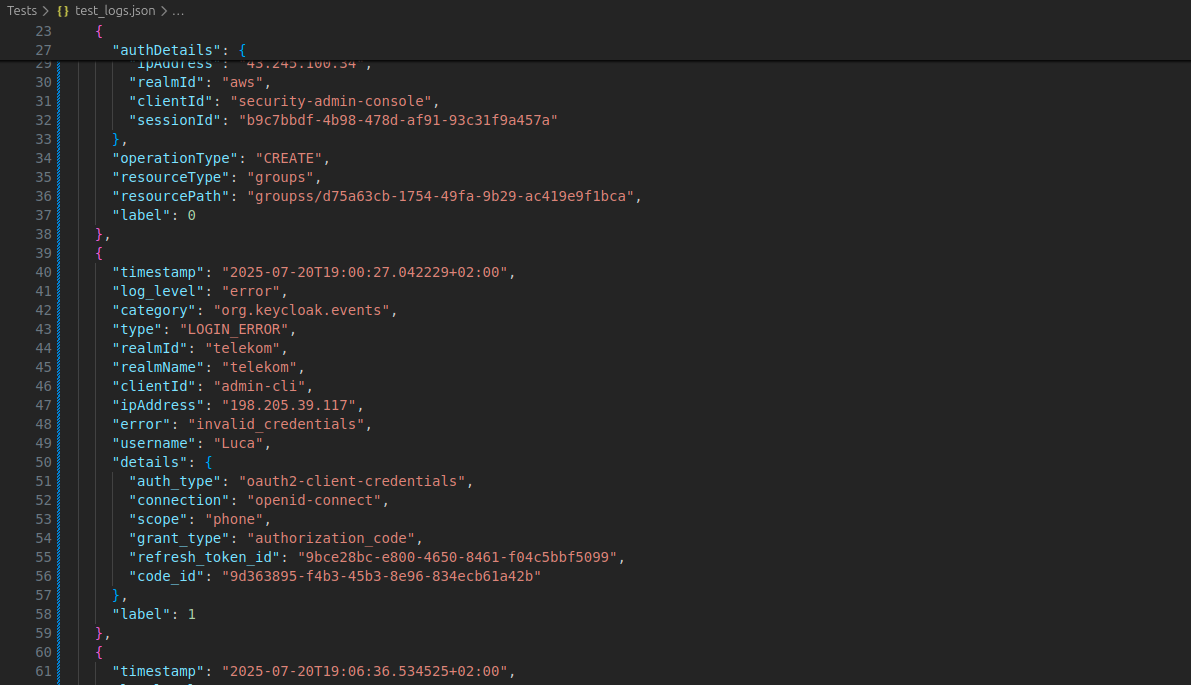
\includegraphics[width=1.0\linewidth]{screenshot009}
		\caption{Ausschnitt der generierten Logs}
		\label{fig:screenshot009}
	\end{figure}
	
	Bei der Generierung der Log-Daten wurde auch beachtet, dass nicht nur Normale und Anormale Benutzer-Sessions erzeugt werden, sondern auch Sessions, welche sich nicht klar zuordnen lassen. Dies wird dann auch \textit{Noise} genannt. Noise tritt des Öfteren in realen Anwendungsfällen auf, weil auch normale Benutzer manchmal bspw. priorisierte Rollen erhalten müssen aus Management-Gründen oder auch zu oft das Passwort ändern aus eigenen Bedenken der Sicherheit. Die Modelle würden dazu tendieren diese als Anormal zu deuten. Dies wird hier verhindert, indem noch im Script mit Absicht Noises erzeugt werden.
	
	\subsection{Problematik dieser Lösung}
	Bei der Generierung der Logs wurden nur die wichtigsten Features erzeugt, welche auf notwendig, sind um Anomalien zu finden. Im Rahmen der Arbeit war es nicht möglich, detaillierte Informationen über die genaue Anlage und Struktur der Event Typen im Keycloak-System zu erhalten, da hierzu keine umfassende Dokumentation vorlag und der Zugriff auf administrative Ressourcen eingeschränkt war. Daher wurde die Analyse auf die verfügbaren und typischen Log-Daten gestützt, die generische Features und Muster der Systemaktivitäten widerspiegeln. Diese Einschränkung wird im weiteren Verlauf berücksichtigt und limitiert die Tiefe der Auswertung.
	\\[0.5em]
	Eine Herausforderung dieser Arbeit war, die Wahrscheinlichkeit zu bestimmen, wann eine Session Anormal ist, wann normal und wann es einfach Noise, also normale Logdaten,welche aber Anomalien ähneln, ist. Da Anomalien selten sind wurde ein Wert für die Wahrscheinlichkeit des Auftretens einer Anomalie 2 Prozent bestimmt. Da diese Entscheidung auf Intuition basiert, wird nicht gewährleistet, dass die Daten keine realen Daten abbilden können. Dies beeinflusst das Ergebnis.
	\\[0.5em]
	Aufgrund dieser Nachteile und den resultierenden Ergebnissen, wurde dieser Ansatz an den Modellen getestet, wird aber verworfen.
	
	\section{Möglichkeit 2: Datenbeschaffung als Alternative}
	Da die Generierung der Daten eine hohe Aufwendigkeit benötigt, wird stattdessen der sinnvollere Ansatz verwendet, echte Keycloak-Daten zu beschaffen. Jedoch werden es keine Daten aus Unternehmen, da man keine datenschutzrechtlichen Risiken eingehen will. Stattdessen wurde die Idee angenommen, über eine lokale Keycloak-Instanz selbst Log-Daten zu generieren. Da dieser Weg zeitaufwendig ist, wurde in Betracht gezogen, über sogenannte Selenium-Tests Angriffsszenarien zu inszenieren und ebenfalls durch Selenium-Tests gewöhnliche Keycloak-Daten zu generieren. Was dabei als normale Keycloak-Logs zu verstehen ist, wird dadurch  herausgefundenen, sich an firmeninternen Logs zu orientieren.
	
	\subsection{Anbindung der Keycloak-Api}
	Um Zugriff auf die Keycloak-Logs zu erhalten, war es notwendig, selbst eine Keycloak-Instanz aufzusetzen und selbst als Admin zu navigieren. 
	Um nun an die Logs aus Keycloak, also die die aus Quarkus hauptsächlich aus generiert werden, zu kommen, muss man zuerst die benötigten Ressourcen finden. Standard gemäß benötigt man Admin-Rollen, um an sensible Informationen wie User Event Logs und den Admin Event Logs selbst zu gelangen. Man benötigt zunächst einmal die korrekten Authentifizierungsmittel, damit man auch Rechte erlangt, um auf die Events zugreifen zu dürfen.
	\\[0.5em]
	Der gewählte Grant Typ hierfür ist \textit{Client Credentials}. Hierbei meldet man sich über einen beliebigen Client an. man benötigt noch das Client-Secret und schickt dieses mit den anderen Daten ab.
	\\[0.5em]
	\begin{figure}[H]
		\centering
		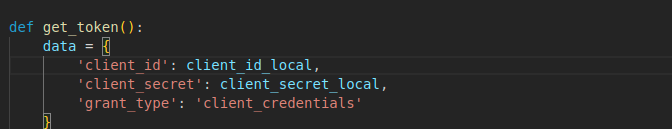
\includegraphics[width=0.9\linewidth]{screenshot010}
		\caption{Daten, die an den Keycloak-Server gesendet werden müssen}
		\label{fig:screenshot010}
	\end{figure}
	Man erhält dadurch den Token, welcher benötigt wird, um nun an die Event Logs zu importieren. Im Token sind die Zugriffsrechte geschildert, die der jeweilige Admin hat, er benötigt die Rollen, die dazu benötigt ist, Benutzer zu verwalten,welche dann auch im Token aufgelistet ist. Nun wird eine weitere URL aufgerufen, bzw., ein Request wird gestellt, um die Event Logs zu holen, wobei der Token als Autorisierungsnachweis mitgegeben wird. Die geladenen Event Logs werden danach in einer separaten JSON-Datei gespeichert.
	\\[0.5em]
	Genauere Informationen über die Keycloak API lassen sich in der 
	Doku finden \footnote{https://www.keycloak.org/docs-api/latest/rest-api/index.html}.
	
	\subsection{Selenium-Tests}
	Selenium ist ein Framework für automatisierte Tests im Webbrowser. Selenium-Tests sind als Paket erhältlich in Python. Bei den Selenium-Tests wird der Webbrowser genau, wie als ob  würde ein echter Mensch ihn benutzen, ausgeführt. Der Anwender sieht klar, wie die UI benutzt wird durch den geschriebenen Test. Selenium-Tests bestehen aus folgenden Komponenten:
	\begin{itemize}
		\item Selenium WebDriver: Das Herzstück – steuert den Browser programmgesteuert.
		\item Selenium Grid: Ermöglicht parallele Tests auf mehreren Maschinen/Browsern.
		\item Selenium IDE: Ein Recording-Tool im Browser (nicht empfohlen für ernsthafte Tests).
	\end{itemize}
	Generell wird für die Erstellung der Logs nur der Webdriver verwendet. Dieser führt automatisch den Chrome Browser aus. Der Grund für die Wahl von Selenium beruht auf seine unkomplizierte Anbindung an Keycloak und auch der Tatsache, dass Selenium-Tests auch auf Keycloak anwendbar sind. Die Anbindung an sich erfordert keinen hohen Aufwand; man muss den "Driver", also den Browser, definieren, und daraufhin die Tests ausführen auf dem jeweiligen Port, auf dem die lokale Keycloak-Instanz lauscht.
	\\[0.5em]
	Ein Nachteil der Tests ist, dass die IP-Adresse gleich bleibt und dies ein Störfaktor darstellt. Die Modelle lernen, dass jede IP-Adresse zu verschiedenen Benutzern gehört, obwohl dies in der Realität nicht der Fall ist und auf Anomalien hinweisen sollte. Zudem gibt es Probleme bezüglich der Zeit: Alle Logs werden in einem Durchlauf in leichten Abständen erstellt. Da der LSTM-AE zeitbasiert lernt, wird dies seine Fähigkeit die Anomalien zu erkennen, eingeschränkt. Es werden auch Tests am Abend durchgeführt, jedoch hat man dann auch nur ein paar Anomale Logs, welche auf eine ungewöhnliche Uhrzeit hinweisen. 
	\\[0.5em]
	Dennoch besteht der Vorteil, dass die Logs realitätsnah an den echten Keycloak-Logs ist, was wichtiger ist, falls die Erkenntnisse dieser Arbeit wirtschaftliche Vorteile mitbringen soll. Es lassen sich 100000 Events oder sogar mehr erstellen, womit das LSTM-AE genug Daten zur Verarbeitung hat. Zudem werden automatisch reale Logs durch die Aktionen in den definierten Tests erzeugt, woraufhin keine eigenen Logs mehr generiert werden müssen, sondern die Logs automatisch durch die Selenium-Tests erzeugt werden und gespeichert werden. 
	\\[0.5em]
	
	\begin{figure}[H]
		\centering
		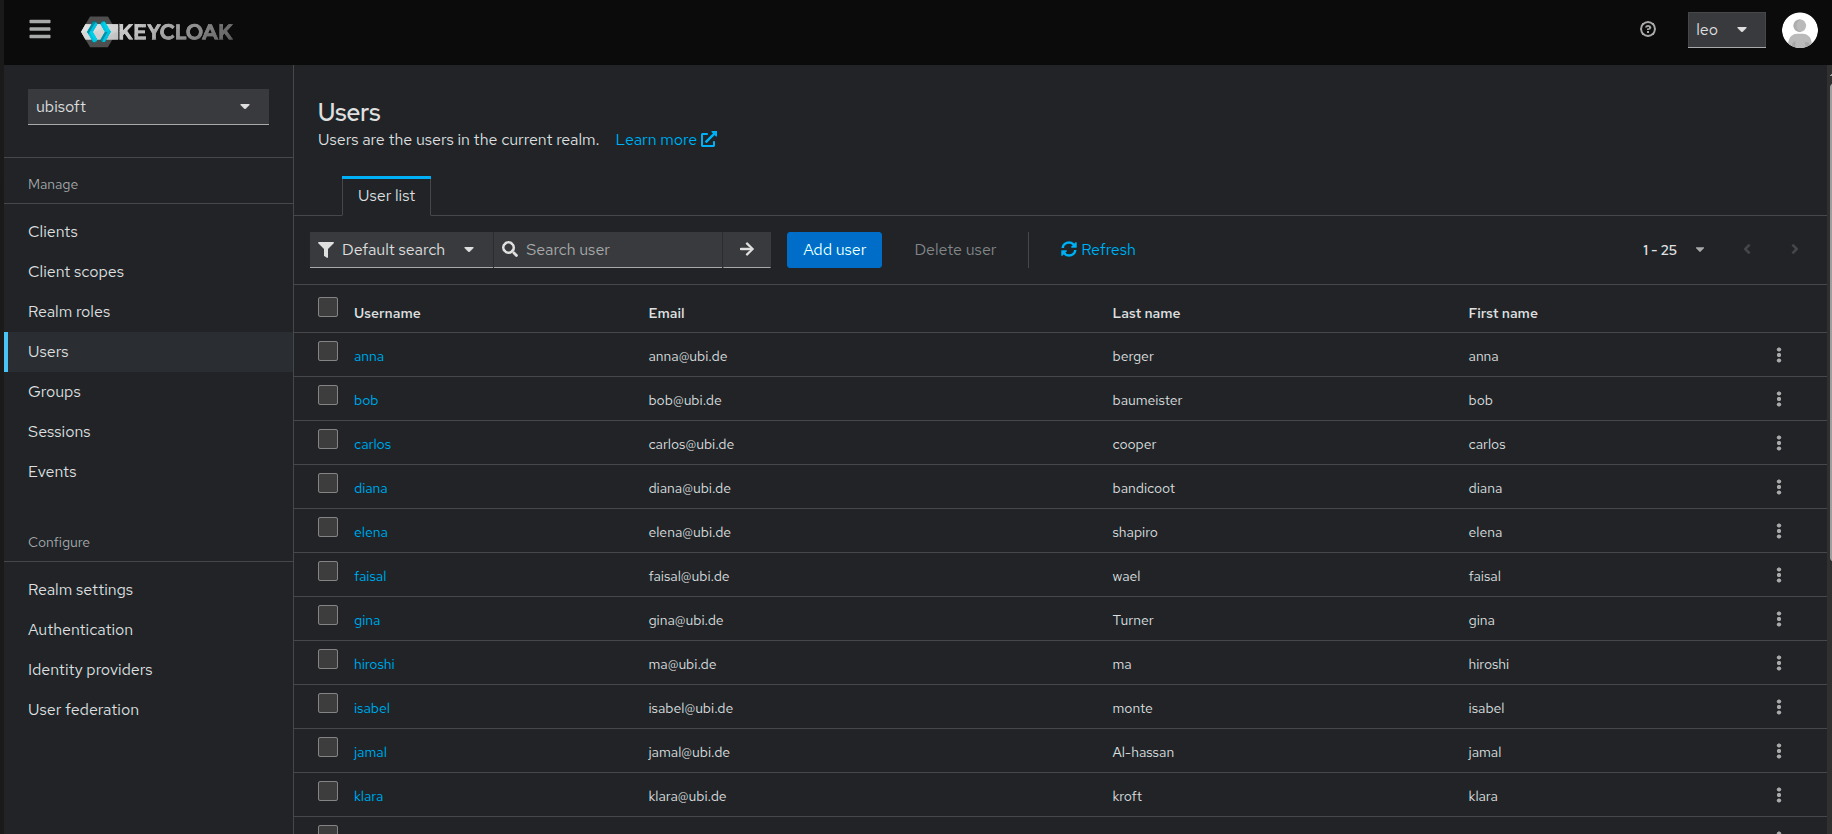
\includegraphics[scale=1.5, width=\linewidth]{screenshot011}
		\caption{Hier sieht man die generierten Benutzer für den Testfall}
		\label{fig:screenshot011}
	\end{figure}
	
	
	Es wurde zur Generierung der normalen Trainingsdaten zuvor ein neuer Realm erstellt namens "Ubisoft". In diesem sind 25 generierte nicht lebende Benutzer, wobei alphabetisch generiert wurde beginnt jeder Name mit je einem Buchstaben des Alphabets außer "X". Es wurde in diesem Realm der Client "nintendo" angelegt.  Dieser ist notwendig für den Admin, um auf die User Events zuzugreifen, als auch für die Benutzer selbst, wenn bspw. ein unechter Benutzer sich mit dem Client "nintendo" anmeldet.
	\\[0.5em]
	Ein Selenium-Test dieser Arbeit, erzeugt automatisch neue Benutzer in Keycloak und setzte zudem ein jeweiliges Passwort. Diese Benutzerdaten mitsamt dem Passwort werden jeweils in einer JSONL-Datei gespeichert und Benutzernamen und Passwort werden jeweils gemeinsam als Wert kombiniert. Damit sich die Benutzer auch über Keycloak über die automatisierten Tests anmelden können, muss in Keycloak eingestellt, dass die Benutzer kein vollständiges Profil mit Vornamen, Nachnamen und E-Mail brauchen, da ansonsten die Anmeldung fehlschlägt.
	\\[0.5em]
	Über einer bestimmten Anzahl für die Trainingsdaten, werden die generierten Benutzer im Selenium-Test dazu gebracht, sich anzumelden. "Gewöhnliche" Logs sind u.A. Logs,welche mit der Anmeldung zu tun haben. Inspiriert wurde dies durch echte firmeninternen Logs, welche hauptsächlich aus den Event-Type  LOGIN, CLIENT\_LOGIN und CODE\_TO\_TOKEN bestehen, wie in den firmeninternen Logs.
	\\[0.5em]
	Im Realm „Ubisoft“ benötigt ein Admin-Benutzer, der für einen bestimmten Client Benutzer erstellen möchte, die Rolle „manage-users“. Zusätzlich ist die Rolle „view-events“ erforderlich, um Ereignisse als Logs speichern und einsehen zu können. Wichtig dabei ist, dass diese Rollen nicht direkt dem Benutzer, sondern dem Client zugewiesen werden. Das liegt daran, dass Clients in Keycloak eigene Zugriffsrechte besitzen, die ihnen erlauben, bestimmte Aktionen im System auszuführen. So braucht der Client beispielsweise die Rolle „manage-users“, um programmgesteuert Benutzer im Realm anlegen oder verwalten zu können. Die Rolle „view-events“ ermöglicht es dem Client, Ereignisse und Logs zu überwachen, was für das Monitoring und die Fehleranalyse essenziell ist.
	\\[0.5em]
	Darüber hinaus verfügen Clients oft über sogenannte Service Accounts, spezielle Benutzerkonten, die es dem Client ermöglichen, sich selbstständig zu authentifizieren, etwa über das OAuth2 Client Credentials Grant. Die Service Account Rollen bestimmen dabei die Rechte, die diesem Service Account zugewiesen sind. Ohne die passenden Service Account Rollen könnte der Client zwar eine Verbindung herstellen, wäre aber nicht berechtigt, Benutzer zu verwalten oder Logs einzusehen. Somit sind die Service Account Rollen entscheidend dafür, dass ein Client im Hintergrund ohne Benutzerinteraktion die notwendigen Operationen ausführen kann.
	\\[0.5em]
	Kurz gesagt: Der Client braucht die Rollen „manage-users“ und „view-events“, um Benutzerverwaltung und Event-Logging durchzuführen, und die Service Account Rollen, damit er sich eigenständig authentifizieren und diese Rechte nutzen kann.
	\\[0.5em]
	\begin{figure}[H]
		\centering
		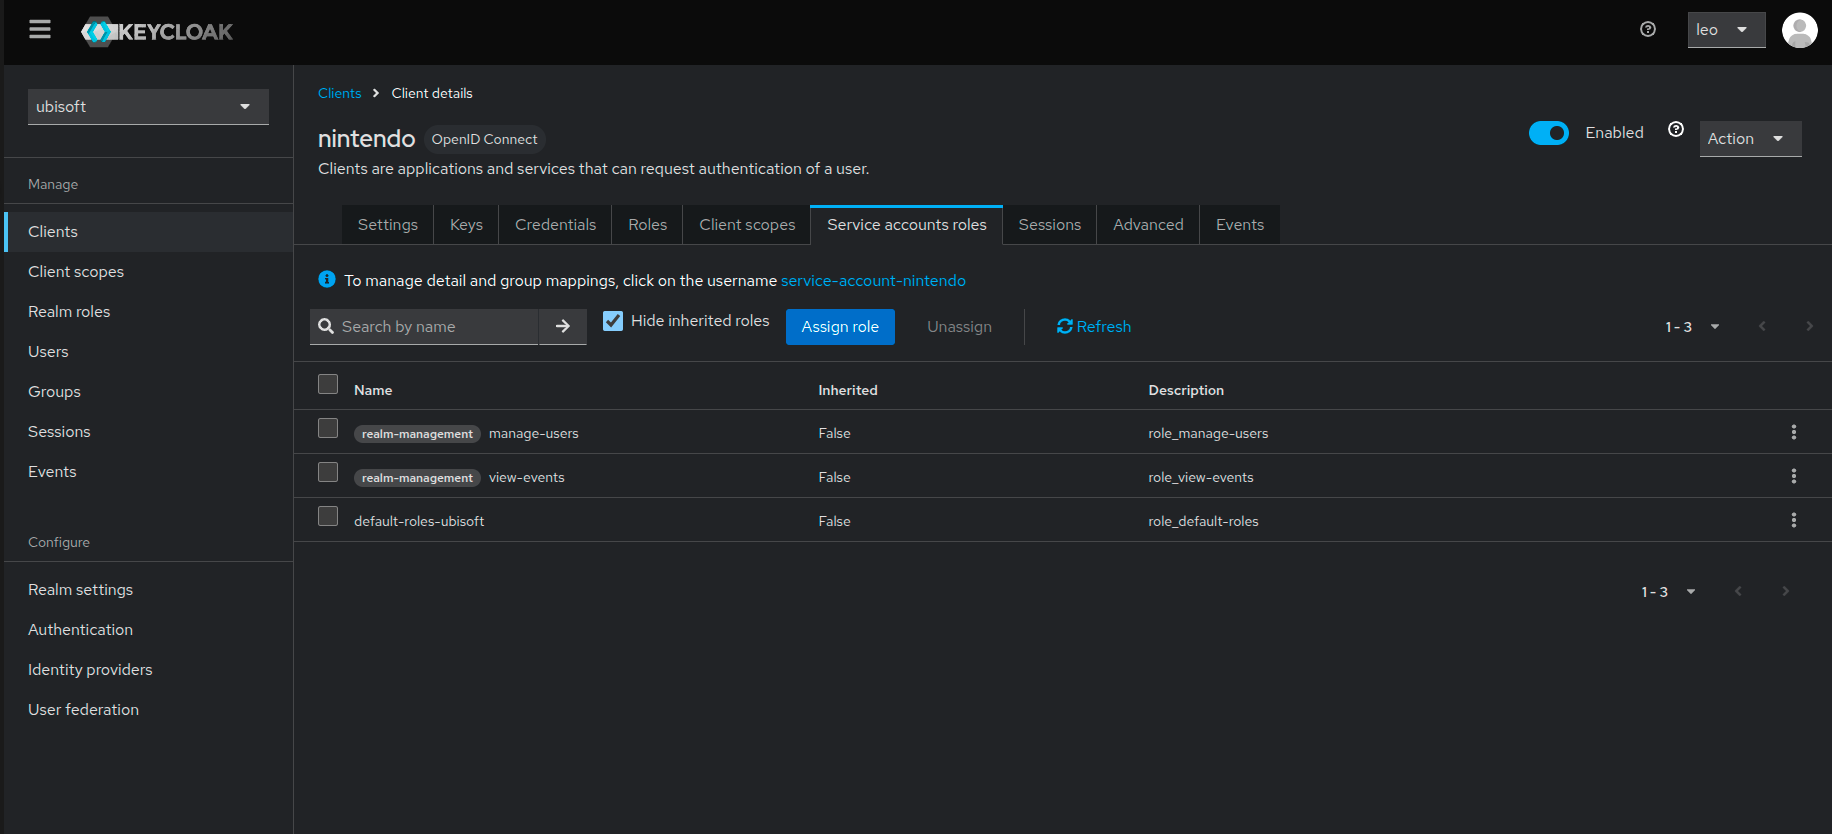
\includegraphics[width=0.9\linewidth]{screenshot012}
		\caption{Benötigte Rollen für den Client Nintendo}
		\label{fig:screenshot012}
	\end{figure}
	
	Es werden ca. 5000 Logs erzeugt, welche nur gewöhnliche Los enthalten mit den genannten Event-Typen. Zudem führt ein weitere Selenium-Test Aktionen aus, die auf die Anomalien hindeuten sollen. Es werden ca. 15-25 solcher Logs erzeugt, wobei drei Szenarien ausgeführt werden. Diese Szenarien werden im nächsten Kapitel genau erläutert und unterscheiden sich von den Anwendungsfällen, welche zuvor bei der Generierung der Logs genannt wurden.
	\\[0.5em]
	
	\subsection{Mögliche Angriffszenarien nach CVE und CWE}
	
	Common Vulnerabilities and Exposures (CVE) stellt eine Auflistung bzw. Datenbank aller bekannten Sicherheitslücken in einem System dar. Für Keycloak existieren ebenfalls zahlreiche dokumentierte Schwachstellen \footnote{\url{https://cve.mitre.org/cgi-bin/cvekey.cgi?keyword=keycloak}}.
	\\[0.5em]
	CVEs bieten jedoch keine Lösungen an, sondern dienen der transparenten und neutralen Information über die Art, Ursache und mögliche Auswirkungen der jeweiligen Sicherheitslücke. Jede CVE erhält eine eindeutige Identifikationsnummer, eine Kurzbeschreibung sowie (sofern verfügbar) Angaben zur betroffenen Softwareversion. Die Dokumentation erfolgt weltweit durch Organisationen, Forschungseinrichtungen und unabhängige Sicherheitsforscher.
	\\[0.5em]
	Common Weakness Enumeration (CWE) hingegen beschreibt systematisch bekannte Schwachstellenmuster (Weaknesses), die potenziell zu Sicherheitslücken führen können. Während CVEs auf bereits konkret ausgenutzte oder gefundene Schwachstellen hinweisen, beschreibt CWE eher abstrakte Klassen von Fehlern, wie z.,B. „unzureichende Rechteprüfung“ oder „unsichere Tokenverarbeitung“. Beide Kataloge sind essentiell, um systematische Sicherheitstests zu entwerfen und zu interpretieren.
	\\[0.5em]
	Im Rahmen dieser Arbeit wurden mit Hilfe von Selenium gezielt sicherheitsrelevante Szenarien gegen Keycloak getestet und simuliert. Dabei lassen sich die folgenden Fälle konkreten CVE- und CWE-Einträgen zuordnen:

	\begin{itemize}
		\item \textbf{Privilege Escalation Test:}
		Bei diesem Test wurde überprüft, ob sich ein normaler Benutzer unbefugt Zugriff auf administrative Bereiche verschaffen kann. Die Logik entspricht dem bekannten Schwachstellenmuster \textbf{CWE-269: Improper Privilege Management}. In Bezug auf Keycloak wurde eine vergleichbare Schwachstelle mit \textbf{CVE-2019-10160} dokumentiert, bei der Benutzer durch unzureichende Prüfung ihrer Rollen Zugriff auf administrative Endpunkte erhalten konnten.
		\item \textbf{Token Manipulation Test:}  
		In diesem Test wurde ein gültiges OAuth2 Access Token manipuliert (z.\,B. durch Abschneiden und Ändern von Zeichen), um zu prüfen, ob das System die Signaturprüfung korrekt durchführt. Die zugrundeliegende Schwachstelle ist unter \textbf{CWE-347: Improper Verification of Cryptographic Signature} klassifiziert. Eine konkrete Verwundbarkeit, bei der ein ähnlicher Fall auftrat, ist \textbf{CVE-2020-13957}, bei dem manipulierte Tokens fälschlicherweise akzeptiert wurden.
		\item \textbf{Denial of Service (DoS) Test:}  
		Mittels zahlreicher, aufeinanderfolgender Anfragen wurde versucht, das System durch Last zu destabilisieren. Diese Art der Schwachstelle fällt unter \textbf{CWE-400: Uncontrolled Resource Consumption}. Eine reale CVE mit Bezug auf Keycloak ist \textbf{CVE-2021-41117}, bei der durch komplexe Gruppenrollenstrukturen ein ressourcenintensiver Zustand ausgelöst werden konnte, was ebenfalls zu einem DoS führen konnte.
	\end{itemize}

	Diese Tests orientieren sich an bekannten Sicherheitslücken und dienen dazu, die Robustheit des Systems unter realistischen Angriffsbedingungen zu validieren. Da CVE- und CWE-Datenbanken bewusst keine vollständigen Exploitbeschreibungen enthalten, musste im Rahmen der Simulation eine technische Interpretation der Schwachstellen erfolgen.
		
	\section{Durchführung des Trainings}
	\subsubsection{Training und Tests bei den Generierten Logs}
	\subsubsection{Training und Tests bei den Logs durch Selenium}
	\section{Ergebnisse}
	\section{Diskussion}
	\section{Fazit}
	\section{Ausblick}
\newpage	
\bibliographystyle{unsrt}
\bibliography{quellen} 
\newpage 
\renewcommand{\notesname}{Fußnotenverzeichnis}
\renewcommand{\enoteformat}{\rightskip0pt\leftskip0pt\vspace{0.5em}\noindent\makebox[2em][l]{\theenmark}}
\theendnotes
\end{document}